\section{Lineare Funktionen – Geraden verstehen}

Nachdem wir gesehen haben, dass der Dreisatz eng mit linearen Zusammenhängen verknüpft ist, wollen wir uns nun systematisch mit \textbf{linearen Funktionen} beschäftigen. Sie sind die einfachste Art von Funktionen, aber unglaublich wichtig als Grundlage für komplexere Modelle.


\begin{tcolorbox}[colback=blue!5!white, colframe=blue!75!black, title=Was du in diesem Kapitel lernen wirst:]
Nachdem du dieses Kapitel durchgearbeitet hast, wirst du in der Lage sein:
\begin{itemize}[noitemsep, topsep=0pt]
    \item zu erklären, was eine lineare Funktion ist und wie ihre allgemeine Form lautet.
    \item die Bedeutung der Parameter $a$ (Steigung) und $b$ (y-Achsenabschnitt) zu verstehen und zu interpretieren.
    \item den Graphen einer linearen Funktion zu zeichnen und aus einem Graphen Informationen abzulesen.
    \item die Steigung einer Geraden aus zwei Punkten zu berechnen.
    \item die Funktionsgleichung einer linearen Funktion aus verschiedenen Angaben (z.B. zwei Punkte, Steigung und ein Punkt) aufzustellen.
    \item Nullstellen linearer Funktionen zu berechnen und zu interpretieren.
    \item Wertetabellen zu erstellen und zu nutzen.
    \item Schnittpunkte von zwei Geraden zu berechnen.
    \item Anwendungsaufgaben mit linearen Funktionen zu modellieren und zu lösen.
    \item das Konzept der durchschnittlichen Änderungsrate zu verstehen.
\end{itemize}
\end{tcolorbox}
\bigskip


\begin{infoboxumgebung}{Was bedeutet 'linear'?}
'Linear' kommt vom lateinischen Wort 'linea', was 'Linie' bedeutet. Eine lineare Funktion stellt also immer eine \textbf{gerade Linie} dar, wenn du sie zeichnest. Denk an ein Lineal – das ist ein gutes Bild für etwas Lineares!
Im Alltag begegnen uns lineare Zusammenhänge oft:
\begin{itemize}
    \item Dein Taschengeld pro Woche (wenn es immer gleich viel ist und du bei Null startest oder einen festen Betrag schon hast).
    \item Die Kosten für Benzin, wenn der Preis pro Liter fest ist und du eine bestimmte Menge tankst (ohne Grundgebühr).
    \item Die Strecke, die du mit konstanter Geschwindigkeit zurücklegst, wenn du die Zeit als Variable nimmst.
    \item Viele Gebührenmodelle: eine feste Grundgebühr plus ein Betrag pro Einheit (z.B. pro Minute telefonieren, pro gefahrenem Kilometer).
\end{itemize}
Lineare Funktionen beschreiben also Situationen, in denen die Änderung einer Größe immer gleichmäßig erfolgt.
\end{infoboxumgebung}

Jetzt wird es etwas formaler, aber keine Sorge, wir erklären alles Schritt für Schritt.

\begin{merksatzumgebung}[Lineare Funktion]{Die allgemeine Form}
Eine lineare Funktion hat die allgemeine Form:
\[ f(x) = a \cdot x + b \]
oder auch oft geschrieben als (besonders in der Geometrie):
\[ y = a \cdot x + b \]
Dabei bedeuten die Buchstaben:
\begin{itemize}
    \item $f(x)$ oder $y$: Der \textbf{Funktionswert} (oder y-Wert). Das ist das Ergebnis, das die Funktion liefert, wenn du einen bestimmten Wert für $x$ einsetzt. Im Koordinatensystem ist das die Höhe des Punktes auf der Geraden.
    \item $x$: Die \textbf{Variable} (oder x-Wert, Argument). Für $x$ kannst du verschiedene Zahlen einsetzen. Im Koordinatensystem ist das die Position auf der horizontalen Achse.
    \item $a$: Die \textbf{Steigung} der Geraden. Sie sagt dir, wie steil die Gerade ansteigt oder abfällt, wenn du auf der x-Achse um eine Einheit nach rechts gehst. Eine positive Steigung bedeutet 'bergauf', eine negative Steigung 'bergab'.
    \item $b$: Der \textbf{y-Achsenabschnitt}. Er sagt dir, an welcher Stelle (bei welchem y-Wert) die Gerade die y-Achse schneidet. Das ist immer der Funktionswert an der Stelle $x=0$, denn $f(0) = a \cdot 0 + b = b$. Der Punkt ist also $(0|b)$.
\end{itemize}
Die Zahlen $a$ und $b$ nennt man auch \textbf{Parameter} der Funktion. Sie bestimmen, wie genau die Gerade aussieht und wo sie liegt.
\end{merksatzumgebung}



\begin{warumwichtigumgebung}{Parameter $a$ und $b$}
\begin{itemize}
    \item \textbf{Die Steigung $a$ ist entscheidend!} Sie beschreibt die \textit{Rate der Veränderung}. In Anwendungsaufgaben ist $a$ oft ein Preis pro Stück, eine Geschwindigkeit, ein Verbrauch pro Kilometer etc. Ein tiefes Verständnis der Steigung ist der Schlüssel zu vielen Problemen.
    \item \textbf{Der y-Achsenabschnitt $b$ ist der Startpunkt!} In vielen Anwendungen ist $b$ ein fester Grundbetrag, ein Anfangsbestand oder ein Wert zu Beginn einer Messung ($x=0$).
\end{itemize}
Wenn du $a$ und $b$ in einer Textaufgabe identifizieren kannst, hast du oft schon die halbe Miete!
\end{warumwichtigumgebung}

Eine lineare Funktion beschreibt also einen eindeutigen Zusammenhang: Jedem $x$-Wert wird genau ein $y$-Wert zugeordnet, und diese Wertepaare $(x|y)$ liegen alle auf einer Geraden.

% Dein bisheriger Code bis zum Ende der merksatzumgebung


\bigskip % Ein kleiner vertikaler Abstand für bessere Lesbarkeit

Bevor wir uns nun genauer anschauen, wie sich die Parameter $a$ (Steigung) und $b$ (y-Achsenabschnitt) auf den Graphen einer linearen Funktion auswirken und wie wir mit ihnen rechnen, wollen wir noch einmal einen Schritt zurücktreten. Was genau verstehen wir eigentlich unter einer \textbf{Funktion}? Du hast diesen Begriff sicher schon oft gehört, aber eine klare und vielseitige Vorstellung davon ist Gold wert, nicht nur für lineare Funktionen, sondern für alles, was in der Mathematik noch kommt!

\begin{infoboxumgebung}{Was ist eigentlich eine Funktion? – Eine vielseitige Zuordnung}
Ganz grundlegend ist eine Funktion eine Art \textbf{Zuordnungsvorschrift}. Sie nimmt sich etwas aus einer Menge (der sogenannten \textbf{Definitionsmenge}, z.B. Zahlen, die du einsetzen darfst) und ordnet diesem \textbf{eindeutig} etwas aus einer anderen Menge zu (der sogenannten \textbf{Wertemenge}, z.B. die Ergebnis-Zahlen). Stell es dir so vor: Für jede erlaubte Eingabe gibt es genau eine festgelegte Ausgabe.

Hier sind verschiedene Bilder und Ideen, die dir helfen, das Konzept „Funktion“ besser zu greifen:

\paragraph{0. Die Rezept-Analogie: Portionen und Mehl}
Stell dir vor, du möchtest Pfannkuchen backen. Dein Rezept sagt: Für eine Portion Pfannkuchen benötigst du 100 Gramm Mehl.
\begin{itemize}
    \item Für \textbf{1 Portion} ($x=1$) brauchst du $1 \cdot 100\,\text{g} = \mathbf{100\,\textbf{g}}$ Mehl.
    \item Für \textbf{3 Portionen} ($x=3$) brauchst du $3 \cdot 100\,\text{g} = \mathbf{300\,\textbf{g}}$ Mehl.
    \item Für eine \textbf{halbe Portion} ($x=0,5$) brauchst du $0,5 \cdot 100\,\text{g} = \mathbf{50\,\textbf{g}}$ Mehl.
\end{itemize}
Die Anzahl der Portionen (deine Eingabe $x$) bestimmt eindeutig, wie viel Mehl (deine Ausgabe $f(x)$) du benötigst. Als Funktionsgleichung könnten wir schreiben: $f(x) = 100 \cdot x$. Die Funktion $f$ ordnet also der Anzahl der Portionen $x$ die benötigte Mehlmenge $100x$ zu.

\paragraph{1. Die Funktionsmaschine}
Eine sehr beliebte und hilfreiche Vorstellung ist die einer \textbf{Maschine}:
\begin{itemize}
    \item \textbf{Eingabe (Input):} Du wirfst eine Zahl (unser $x$) oben in die Maschine hinein.
    \item \textbf{Verarbeitung:} Im Inneren der Maschine wird mit dieser Zahl nach einer festen Regel etwas Bestimmtes gemacht – sie wird zum Beispiel verdoppelt ($f(x)=2x$), es wird eine Zahl addiert ($f(x)=x+5$), oder es werden mehrere Rechenschritte kombiniert (z.B. $f(x) = 2 \cdot (x+2) + 3$). Diese Regel ist die \textbf{Funktionsvorschrift}.
    \item \textbf{Ausgabe (Output):} Unten kommt genau eine neue Zahl (unser Funktionswert $f(x)$ oder $y$) heraus.
\end{itemize}
Für jede erlaubte Eingabe $x$ liefert die Maschine also eine eindeutig bestimmte Ausgabe $f(x)$.
% Hier könntest du später eine kleine Skizze einfügen, z.B.:
% \begin{center} \includegraphics[width=0.4\textwidth]{pfad/zu/deiner/skizze.png} \end{center}
% (Eine einfache Box mit 'x rein', 'f(x) raus' und 'Rechenregel' in der Mitte)

\paragraph{2. Der (ideale) Getränkeautomat}
Ein bisschen wie ein Getränkeautomat (der immer funktioniert und nie leer ist und nichts kostet \smiley{}):
\begin{itemize}
    \item \textbf{Eingabe:} Du drückst eine Taste (z.B. Taste Nr. 1 für 'Apfelschorle'). Die Tastenwahl ist dein $x$.
    \item \textbf{Ausgabe:} Du erhältst ein bestimmtes Getränk (z.B. eine Apfelschorle). Das Getränk ist dein $f(x)$.
\end{itemize}
Wichtig ist hier: \textbf{Jede Taste ist genau einem Getränk zugeordnet.} Es kann nicht sein, dass du Taste 1 drückst und mal eine Cola, mal eine Limo bekommst. Das ist das Prinzip der \textbf{Eindeutigkeit} einer Funktion! (Es kann aber sein, dass verschiedene Tasten zum selben Getränk führen – z.B. Taste 1 und Taste 5 geben beide Apfelschorle. Das ist bei Funktionen auch erlaubt: Unterschiedliche $x$-Werte können denselben $f(x)$-Wert haben. Aber ein $x$-Wert darf nicht mehrere verschiedene $f(x)$-Werte haben!)

\paragraph{3. Die mathematische Sicht: Eine Abbildung}
In der Mathematik nennt man eine Funktion oft auch eine \textbf{Abbildung}. Sie bildet Elemente einer Menge auf Elemente einer anderen Menge ab.
Wenn wir zum Beispiel sagen, dass wir für $x$ beliebige reelle Zahlen (die Zahlen, die du vom Zahlenstrahl kennst, inklusive Brüchen, Wurzeln etc., geschrieben als $\mathbb{R}$) einsetzen dürfen und als Ergebnis auch wieder reelle Zahlen erhalten, schreiben Mathematiker das manchmal so:
\[ f: \mathbb{R} \to \mathbb{R} \]
Das liest sich als: 'Die Funktion $f$ bildet von den reellen Zahlen in die reellen Zahlen ab.'
Die genaue Vorschrift, was mit einem $x$ passiert, schreibt man dann oft mit einem Pfeil mit einem senkrechten Strich am Anfang:
\[ x \mapsto f(x) \]
Für eine lineare Funktion wie $f(x) = 3x + 1$ würde das bedeuten:
\[ x \mapsto 3x + 1 \]
Das ist einfach eine kompakte Art zu sagen: 'Nimm ein beliebiges $x$, multipliziere es mit 3 und addiere dann 1.'

Das Wichtigste ist: Eine Funktion ist eine \textbf{eindeutige Zuordnung}. Zu jeder Eingabe (aus dem erlaubten Bereich) gibt es genau eine Ausgabe.
\end{infoboxumgebung}

Jetzt, wo wir eine bessere Vorstellung davon haben, was eine Funktion allgemein ist, können wir uns ein paar typische Aufgabenstellungen rund um diese Funktionsmaschinen ansehen.

\begin{aufgabenumgebung}{Funktionsmaschinen-Logik}{}
Stell dir die folgenden Funktionsmaschinen vor. Gib jeweils die Funktionsgleichung $f(x) = \dots$ an, die beschreibt, was die Maschine mit der Eingabe $x$ macht.
\begin{enumerate}
    \item Maschine M1: Verdoppelt die Eingabe $x$ und addiert anschließend 5.
    \item Maschine M2: Subtrahiert von der Eingabe $x$ die Zahl 7 und multipliziert das Ergebnis mit 3.
    \item Maschine M3: Multipliziert die Eingabe $x$ mit sich selbst (quadriert sie) und zieht dann 4 ab.
    \item Maschine M4: Addiert zur Eingabe $x$ die Zahl 2, dividiert das Ergebnis durch 4 und addiert dann $x$.
\end{enumerate}
\end{aufgabenumgebung}

\begin{aufgabenumgebung}{Werte aus der Maschine}{}
Gegeben sind die folgenden Funktionsmaschinen durch ihre Funktionsgleichungen. Welche Ausgabe $f(x)$ (oder $y$) erzeugt die Maschine, wenn die angegebene Zahl $x$ eingegeben wird?
\begin{enumerate}
    \item $f(x) = 4x - 7$
    \begin{itemize}
        \item Was kommt raus bei $x=3$?
        \item Was kommt raus bei $x=0$?
        \item Was kommt raus bei $x=-2$?
    \end{itemize}
    \item $g(x) = -2(x+3)$
    \begin{itemize}
        \item Was kommt raus bei $x=1$?
        \item Was kommt raus bei $x=-3$?
        \item Was kommt raus bei $x=-5$?
    \end{itemize}
\end{enumerate}
\end{aufgabenumgebung}

\begin{erinnerungsboxumgebung}{Grundrechenarten, Vorzeichen und Brüche}
Für lineare Funktionen und das Umstellen von Gleichungen brauchen wir ein paar grundlegende Rechenregeln immer wieder. Das gilt besonders für Steigungen, wo oft Brüche auftauchen. Lass uns kurz checken, ob alles sitzt!

\paragraph{1. Multiplikation und Division mit Vorzeichen}
Beim Multiplizieren und Dividieren von Zahlen mit unterschiedlichen Vorzeichen gilt:
\begin{itemize}
    \item \textbf{Gleiche Vorzeichen:} Das Ergebnis ist \textbf{positiv (+)}.
    \begin{itemize}
        \item $(+) \cdot (+) = (+)$, z.B. $3 \cdot 4 = 12$
        \item $(-) \cdot (-) = (+)$, z.B. $(-3) \cdot (-4) = 12$
        \item $(+) : (+) = (+)$, z.B. $10 : 2 = 5$
        \item $(-) : (-) = (+)$, z.B. $(-10) : (-2) = 5$
    \end{itemize}
    \item \textbf{Unterschiedliche Vorzeichen:} Das Ergebnis ist \textbf{negativ (-)}.
    \begin{itemize}
        \item $(+) \cdot (-) = (-)$, z.B. $3 \cdot (-4) = -12$
        \item $(-) \cdot (+) = (-)$, z.B. $(-3) \cdot 4 = -12$
        \item $(+) : (-) = (-)$, z.B. $10 : (-2) = -5$
        \item $(-) : (+) = (-)$, z.B. $(-10) : 2 = -5$
    \end{itemize}
\end{itemize}

\paragraph{2. Minus vor der Klammer / Subtraktion einer negativen Zahl}
Ein Minuszeichen vor einer Zahl oder Klammer kehrt das Vorzeichen um. Besonders wichtig:
\begin{itemize}
    \item $a - (-b) = a + b$
    \item Beispiel: $7 - (-5) = 7 + 5 = 12$
    \item Beispiel: $-2 - (-8) = -2 + 8 = 6$
\end{itemize}

\paragraph{3. Punkt- vor Strichrechnung}
Denk immer dran: Multiplikation ($\cdot$) und Division (:) werden \textbf{vor} Addition (+) und Subtraktion (-) ausgeführt.
\begin{itemize}
    \item Regel: Zuerst Klammern, dann Punktrechnung, dann Strichrechnung.
    \item Beispiel 1: $5 + 2 \cdot 3 = 5 + 6 = 11$
    \item Beispiel 2: $(5+2) \cdot 3 = 7 \cdot 3 = 21$
    \item Beispiel 3: $10 - 8 : 2 = 10 - 4 = 6$
\end{itemize}

\paragraph{4. Rechnen mit Brüchen}
Brüche begegnen uns oft, z.B. bei Steigungsdreiecken.
\subparagraph{4.1 Kürzen und Erweitern}
\begin{itemize}
    \item \textbf{Kürzen:} Zähler und Nenner durch dieselbe Zahl (außer 0) teilen. Der Wert des Bruchs ändert sich nicht.
    \textit{Formel:} $\frac{a \cdot k}{b \cdot k} = \frac{a}{b}$
    Beispiel: $\frac{6}{9} = \frac{6:3}{9:3} = \frac{2}{3}$
    \item \textbf{Erweitern:} Zähler und Nenner mit derselben Zahl (außer 0) multiplizieren. Der Wert des Bruchs ändert sich nicht.
    \textit{Formel:} $\frac{a}{b} = \frac{a \cdot k}{b \cdot k}$
    Beispiel: $\frac{2}{3} = \frac{2 \cdot 4}{3 \cdot 4} = \frac{8}{12}$
\end{itemize}

\subparagraph{4.2 Addition und Subtraktion von Brüchen}
\begin{itemize}
    \item \textbf{Gleicher Nenner:} Zähler addieren/subtrahieren, Nenner beibehalten.
    \textit{Formeln:} $\frac{a}{c} + \frac{b}{c} = \frac{a+b}{c}$ \quad und \quad $\frac{a}{c} - \frac{b}{c} = \frac{a-b}{c}$
    Beispiel: $\frac{1}{7} + \frac{3}{7} = \frac{1+3}{7} = \frac{4}{7}$
    \item \textbf{Ungleiche Nenner:} Erst auf einen \textbf{gemeinsamen Nenner} (Hauptnenner) erweitern, dann addieren/subtrahieren.
    Beispiel: $\frac{1}{2} - \frac{1}{3} = \frac{1 \cdot 3}{2 \cdot 3} - \frac{1 \cdot 2}{3 \cdot 2} = \frac{3}{6} - \frac{2}{6} = \frac{1}{6}$
\end{itemize}

\subparagraph{4.3 Multiplikation von Brüchen}
\begin{itemize}
    \item Regel: Zähler mal Zähler und Nenner mal Nenner.
    \textit{Formel:} $\frac{a}{b} \cdot \frac{c}{d} = \frac{a \cdot c}{b \cdot d}$
    Beispiel: $\frac{2}{5} \cdot \frac{3}{4} = \frac{2 \cdot 3}{5 \cdot 4} = \frac{6}{20} = \frac{3}{10}$ (Kürzen nicht vergessen!)
\end{itemize}

\subparagraph{4.4 Division von Brüchen}
\begin{itemize}
    \item Regel: Mit dem \textbf{Kehrwert (Reziprokwert)} des zweiten Bruchs multiplizieren.
    \textit{Formel:} $\frac{a}{b} : \frac{c}{d} = \frac{a}{b} \cdot \frac{d}{c} = \frac{a \cdot d}{b \cdot c}$
    Beispiel: $\frac{2}{3} : \frac{5}{7} = \frac{2}{3} \cdot \frac{7}{5} = \frac{2 \cdot 7}{3 \cdot 5} = \frac{14}{15}$
    \item Einen \textbf{Doppelbruch} löst du ebenfalls so auf: $\frac{\frac{a}{b}}{\frac{c}{d}} = \frac{a}{b} : \frac{c}{d} = \frac{a}{b} \cdot \frac{d}{c}$
    Beispiel: $\frac{\frac{1}{2}}{\frac{3}{4}} = \frac{1}{2} \cdot \frac{4}{3} = \frac{4}{6} = \frac{2}{3}$
\end{itemize}


\textbf{Kurze Übungen dazu:}
Berechne die folgenden Terme.
\begin{multicols}{3}
\begin{enumerate}[label=(\alph*)]
    \item $(-5) \cdot 6 = ?$
    \item $7 \cdot (-3) = ?$
    \item $(-8) \cdot (-4) = ?$
    \item $12 : (-3) = ?$
    \item $(-21) : 7 = ?$
    \item $(-30) : (-5) = ?$
    \item $9 - (-4) = ?$
    \item $-6 - (-10) = ?$
    \item $3 - (-3) + (-3) = ?$
    \item $4 + 6 \cdot (-2) = ?$
    \item $15 : 3 - 7 = ?$
    \item $(-2) \cdot (5 - 1) = ?$
    \item $20 - (-5) \cdot 2 = ?$
    \item $18 : (-3) - (-4) = ?$
    \item $\frac{3}{8} + \frac{2}{8} = ?$
    \item $\frac{5}{6} - \frac{1}{3} = ?$
    \item $\frac{2}{5} \cdot \frac{3}{4} = ?$
    \item $\frac{3}{7} : \frac{2}{5} = ?$
    \item $3 \cdot \frac{2}{11} = ?$
    \item $(-\frac{1}{3}) \cdot \frac{2}{5} = ?$
    \item $\frac{4}{5} + (-\frac{1}{2}) = ?$
    \item $(-\frac{2}{3}) : (-\frac{4}{9}) = ?$
    \item $\frac{\frac{2}{5}}{\frac{3}{10}} = ?$
    \item $1 - \frac{3}{5} \cdot \frac{5}{9} = ?$
\end{enumerate}
\end{multicols}

Wenn du bei diesen Aufgaben sicher bist, fällt dir der Umgang mit Termen und Gleichungen bei linearen Funktionen gleich viel leichter!
\end{erinnerungsboxumgebung}


\subsection{Grafische Darstellung – Wie sieht eine lineare Funktion aus?}

Wie schon gesagt: Der Graph (die zeichnerische Darstellung) einer linearen Funktion ist immer eine Gerade. Die Parameter $a$ und $b$ bestimmen ihr Aussehen:

\begin{itemize}
    \item \textbf{Die Steigung $a$ bestimmt die Richtung und Neigung:}
        \begin{itemize}
            \item Ist $a > 0$ (positiv), \textbf{steigt} die Gerade an (wenn man von links nach rechts schaut). Je größer $a$, desto steiler steigt sie.
            \item Ist $a < 0$ (negativ), \textbf{fällt} die Gerade ab. Je kleiner $a$ (d.h. je größer der Betrag von $a$), desto steiler fällt sie.
            \item Ist $a = 0$, ist die Gerade \textbf{waagerecht} (parallel zur x-Achse). Die Funktion ist dann $f(x)=b$, also eine konstante Funktion. Jeder x-Wert hat denselben y-Wert $b$.
        \end{itemize}
    \item \textbf{Der y-Achsenabschnitt $b$ bestimmt die Lage:}
        Er gibt an, wo die Gerade die y-Achse schneidet. Eine Änderung von $b$ verschiebt die Gerade parallel nach oben oder unten.
\end{itemize}

Hier sind einige Beispiele grafisch dargestellt:
\begin{center} % Zentriert den Inhalt
    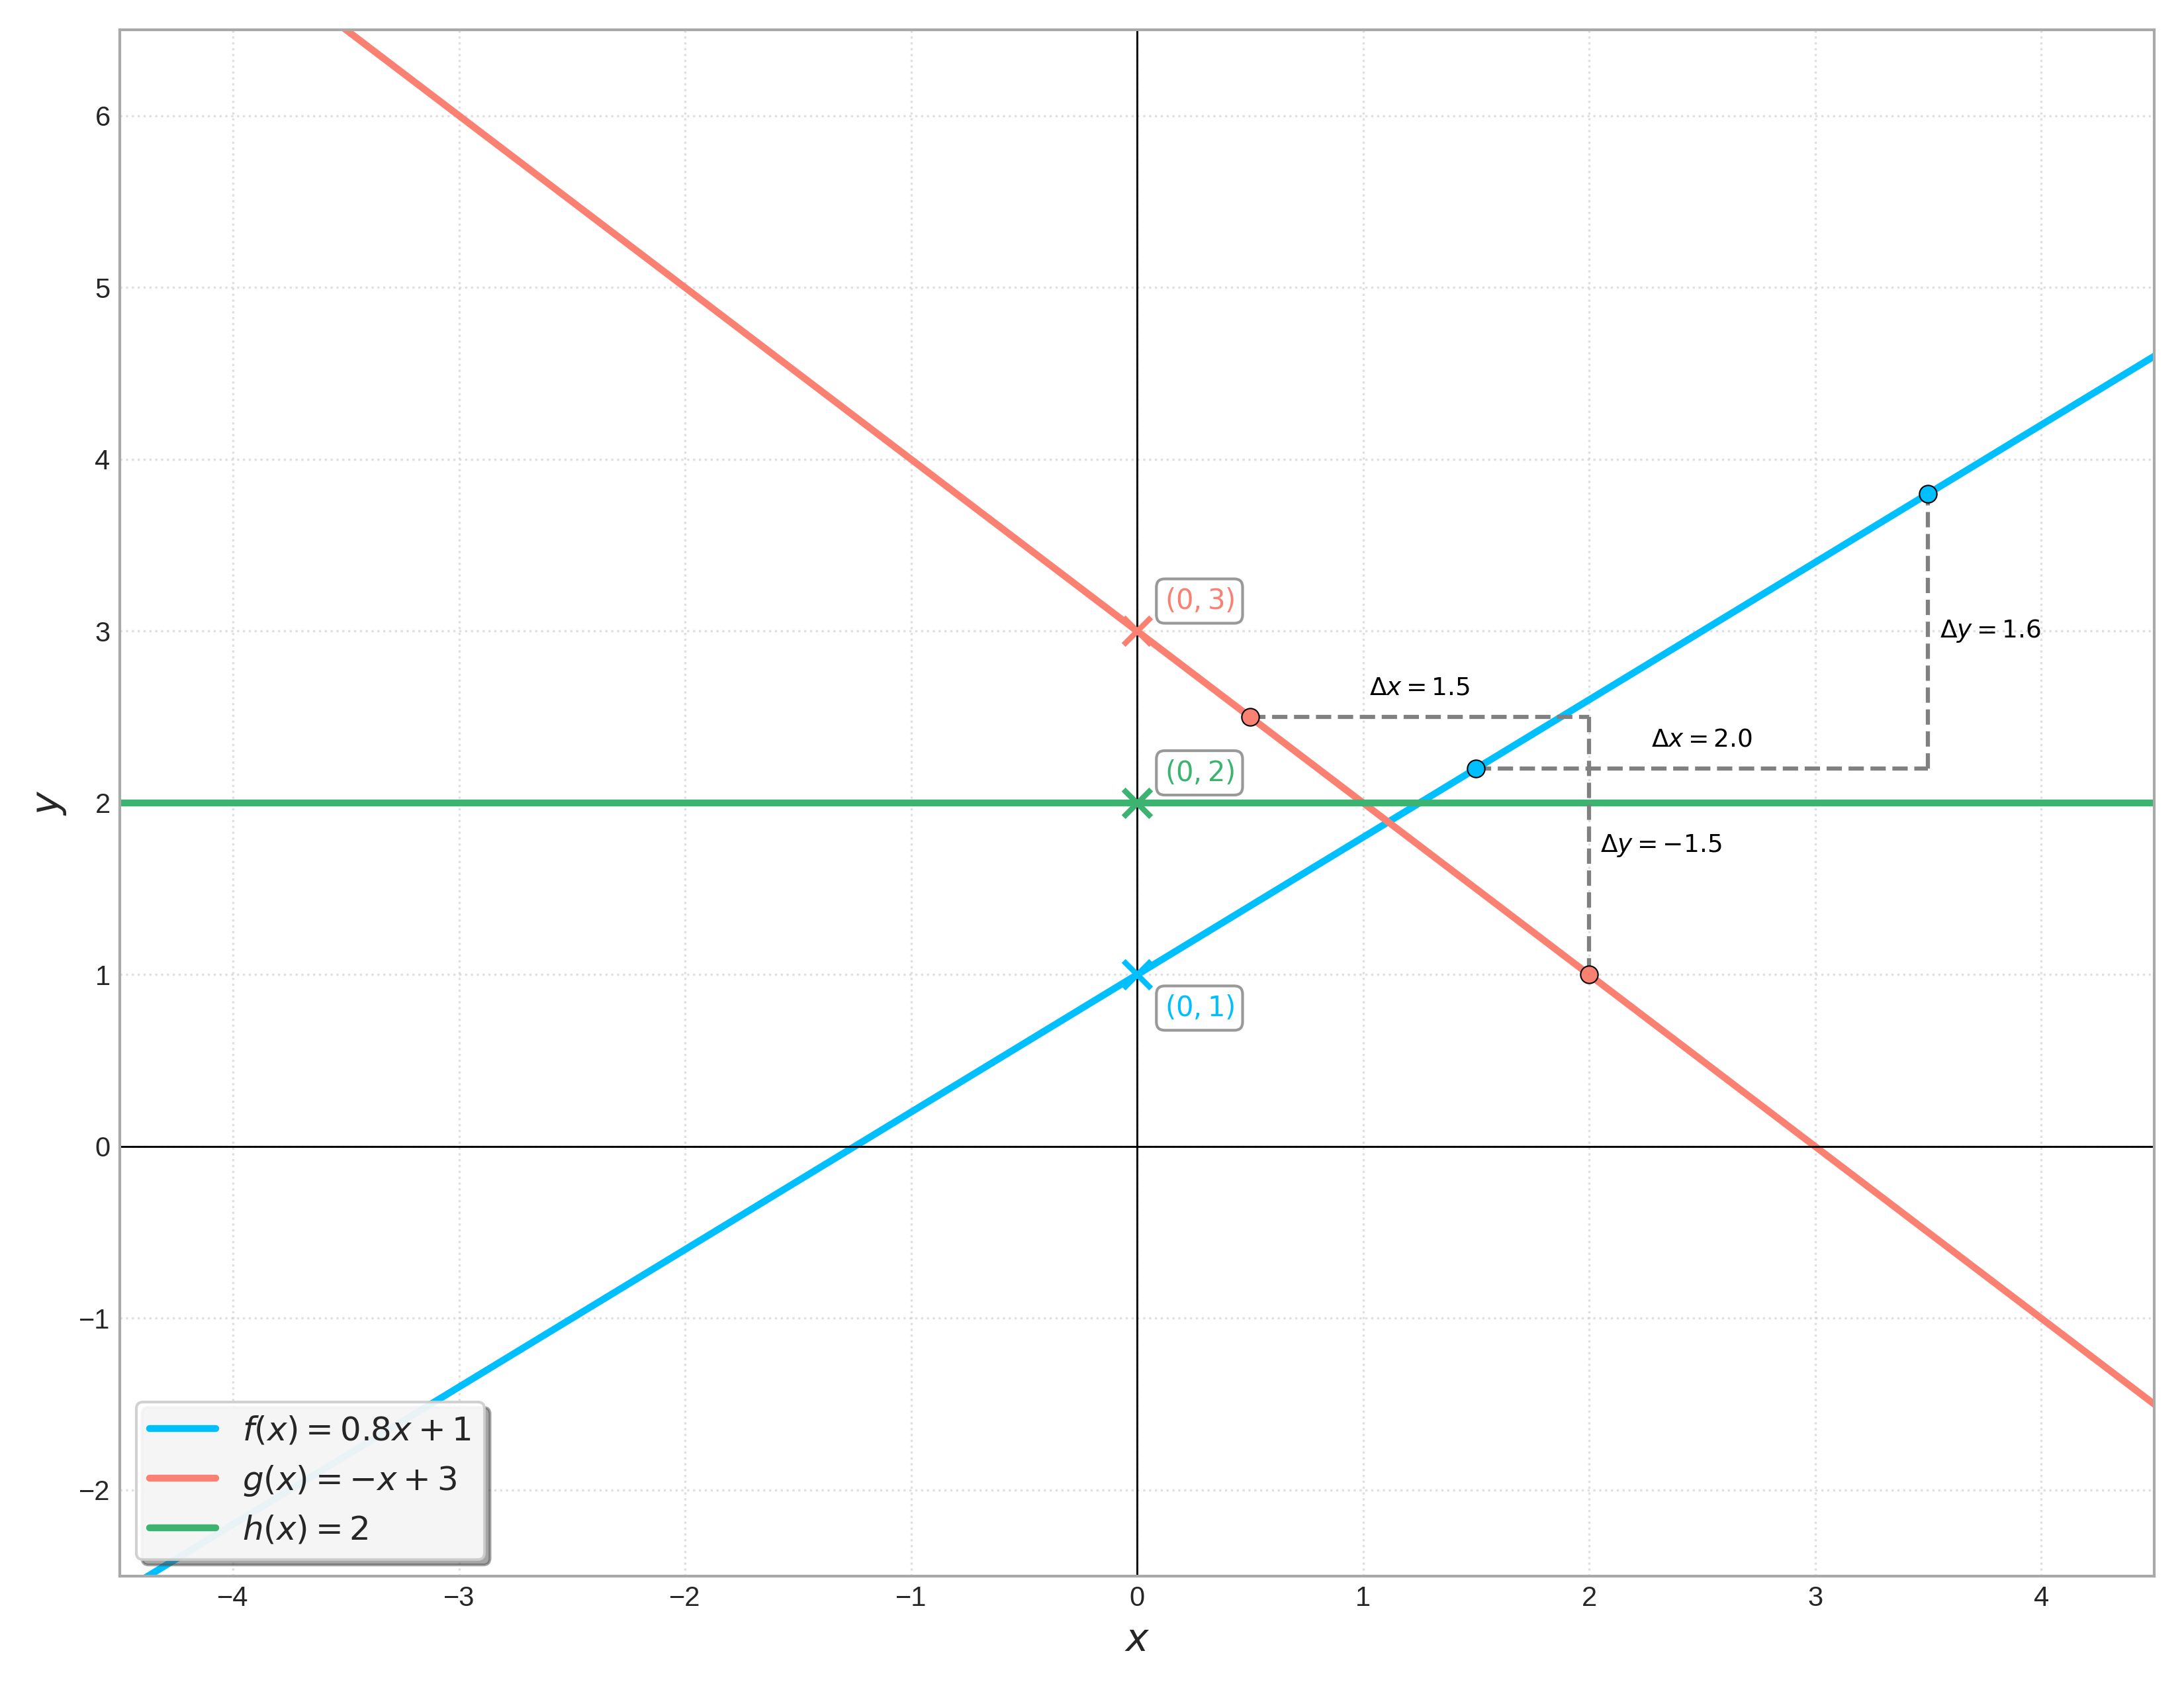
\includegraphics[scale=0.5]{grafiken/Lineare_Funktionen_Beispiele.png}
    \captionof{figure}{Beispiele für lineare Funktionen mit unterschiedlichen Steigungen und y-Achsenabschnitten}
    \label{fig:lineare_funktionen_beispiele}
\end{center}
% Der Text geht hier direkt weiter


Es ist sehr hilfreich, wenn du dir vorstellen kannst, wie sich die Gerade verändert, wenn du $a$ oder $b$ variierst.

\begin{infoboxumgebung}{Trick zum Zeichnen einer Geraden (mit $a$ und $b$):}
Um eine Gerade $f(x)=ax+b$ schnell zu zeichnen, brauchst du nur zwei Punkte. So findest du sie leicht:
\begin{enumerate}
    \item \textbf{Der y-Achsenabschnitt $b$:} Markiere den Punkt $P_1(0|b)$ auf der y-Achse. Das ist dein erster Punkt, denn für $x=0$ ist $f(0)=b$.
    \item \textbf{Das Steigungsdreieck für $a$:} Die Steigung $a$ kannst du oft als Bruch schreiben, z.B. $a = \frac{\Delta y}{\Delta x}$ (Veränderung in y-Richtung geteilt durch Veränderung in x-Richtung).
        \begin{itemize}
            \item Gehe vom Punkt $P_1(0|b)$ aus $\Delta x$ Einheiten nach \textbf{rechts} (entlang der x-Achse).
            \item Von dort gehe $\Delta y$ Einheiten nach \textbf{oben} (wenn $a$ positiv ist, also $\Delta y > 0$) oder $\Delta y$ Einheiten nach \textbf{unten} (wenn $a$ negativ ist, also $\Delta y < 0$).
            \item Der Punkt, den du so erreichst, ist dein zweiter Punkt $P_2$.
        \end{itemize}
        Beispiele für das Steigungsdreieck:
        \begin{itemize}
            \item $a = 2 = \frac{2}{1}$: Gehe 1 nach rechts, 2 nach oben.
            \item $a = -0.5 = -\frac{1}{2} = \frac{-1}{2}$: Gehe 2 nach rechts, 1 nach unten.
            \item $a = \frac{3}{4}$: Gehe 4 nach rechts, 3 nach oben.
        \end{itemize}
        Wenn $a$ eine ganze Zahl ist (z.B. $a=3$), kannst du sie als Bruch $a = \frac{a}{1}$ schreiben (also 1 nach rechts, $a$ nach oben/unten).
    \item \textbf{Verbinden:} Zeichne eine Gerade durch die beiden Punkte $P_1$ und $P_2$. Fertig!
\end{enumerate}
Dieser 'Zeichentrick' ist sehr nützlich!
\end{infoboxumgebung}

Die Steigung ist ein zentrales Konzept, nicht nur bei linearen Funktionen. Schauen wir sie uns genauer an.

\subsection{Die Steigung $a$ – Wie steil ist es?}

Die Steigung $a$ gibt an, um wie viele Einheiten sich der y-Wert ändert, wenn der x-Wert um eine Einheit zunimmt.

\begin{merksatzumgebung}[Steigung berechnen]{Die Steigung $a$ aus zwei Punkten}
Wenn eine Gerade durch zwei gegebene Punkte $P_1(x_1|y_1)$ und $P_2(x_2|y_2)$ verläuft, kannst du ihre Steigung $a$ wie folgt berechnen:
\[ a = \frac{\text{Unterschied der y-Werte}}{\text{Unterschied der x-Werte}} = \frac{y_2 - y_1}{x_2 - x_1} = \frac{\Delta y}{\Delta x} \]
Das Symbol $\Delta$ (Delta, ein griechischer Buchstabe, oft als Dreieck geschrieben) steht in der Mathematik häufig für eine 'Differenz' oder einen 'Unterschied'.
Die Formel $a = \frac{\Delta y}{\Delta x}$ ist fundamental. Man kann sie sich auch als 'Höhenunterschied geteilt durch Längenunterschied' vorstellen, wenn man ein \textbf{Steigungsdreieck} zwischen den beiden Punkten zeichnet.
\end{merksatzumgebung}

Ein Steigungsdreieck ist ein rechtwinkliges Dreieck, das du dir unter (oder über) der Geraden zwischen zwei Punkten vorstellen kannst. Die horizontale Kathete hat die Länge $\Delta x = |x_2-x_1|$ und die vertikale Kathete die Länge $\Delta y = |y_2-y_1|$. Das Vorzeichen von $a$ ergibt sich dann aus der Richtung.

\begin{beispielumgebung}[Steigungsdreieck]{Steigung aus zwei Punkten berechnen und visualisieren}
Gegeben sind die Punkte $P_1(1|2)$ und $P_2(3|6)$. Wie groß ist die Steigung der Geraden durch diese Punkte?

Wir identifizieren die Koordinaten:
$x_1 = 1, y_1 = 2$
$x_2 = 3, y_2 = 6$

Nun berechnen wir die Differenzen:
Unterschied der y-Werte: $\Delta y = y_2 - y_1 = 6 - 2 = 4$.
Unterschied der x-Werte: $\Delta x = x_2 - x_1 = 3 - 1 = 2$.

Jetzt setzen wir in die Formel für die Steigung ein:
\[ a = \frac{\Delta y}{\Delta x} = \frac{4}{2} = 2 \]
Die Steigung der Geraden ist $a=2$. Das bedeutet: Wenn du auf der Geraden 1 Einheit nach rechts gehst, gehst du 2 Einheiten nach oben.

\begin{center}
    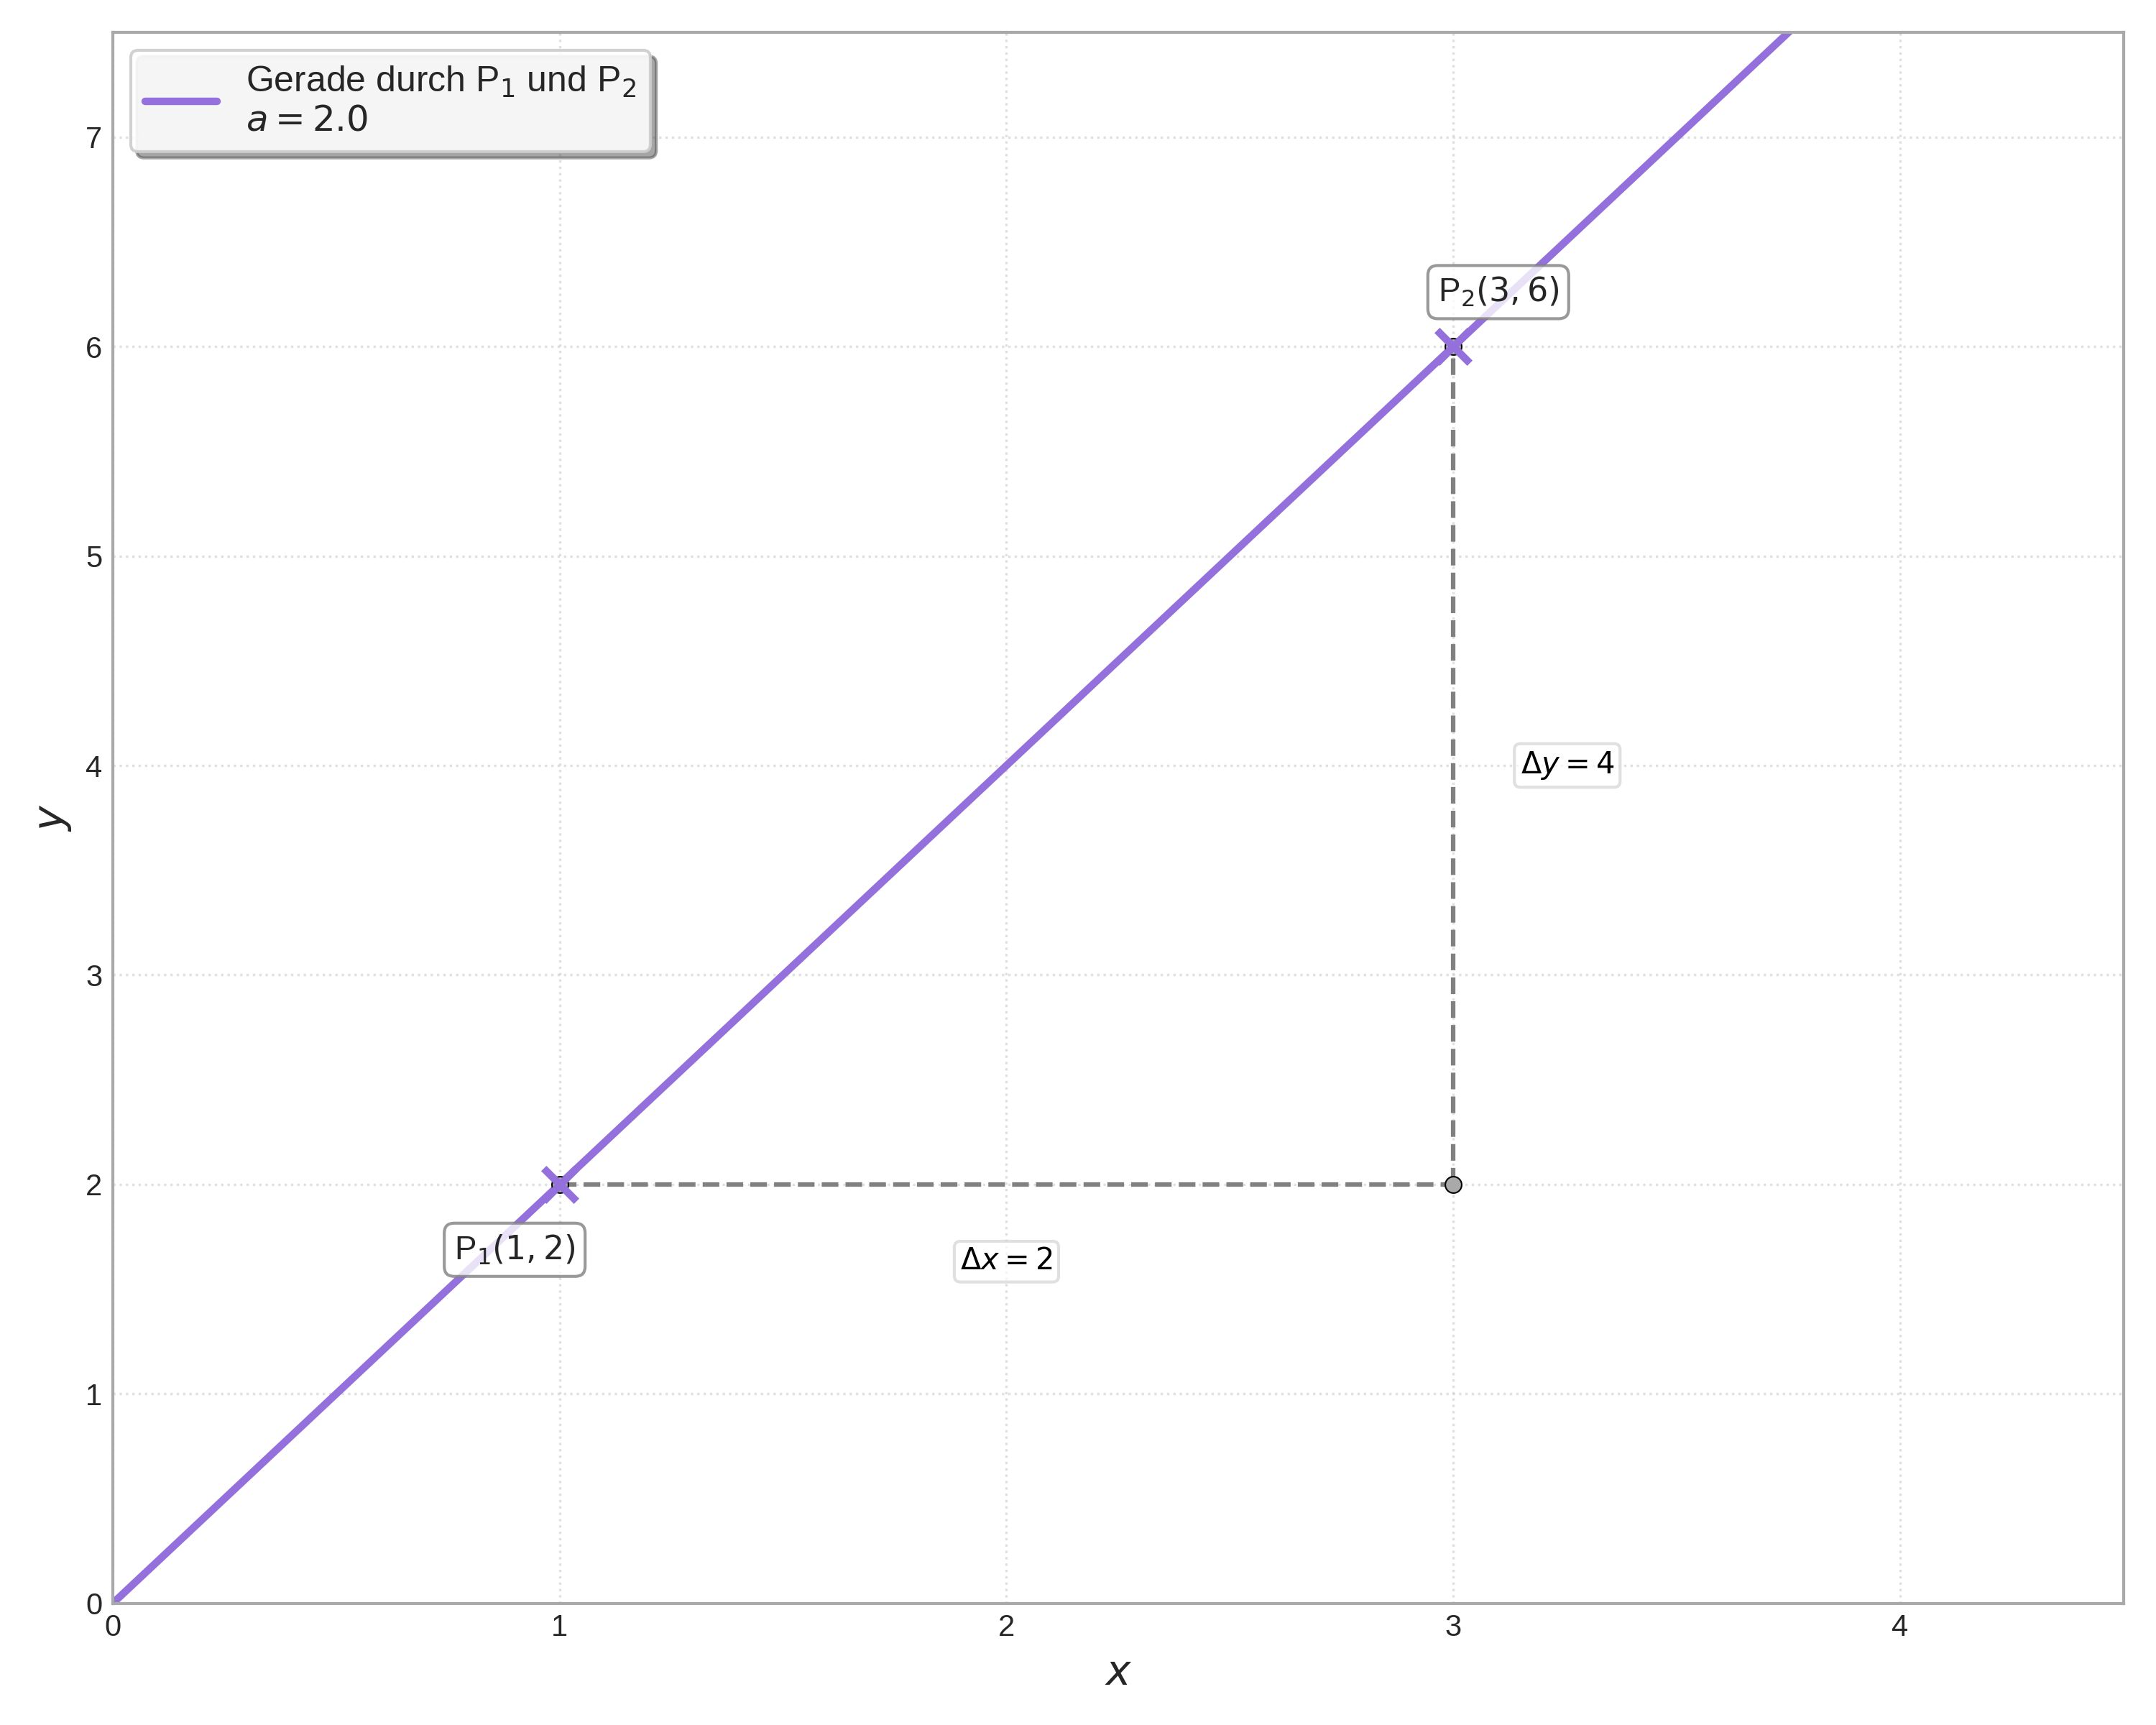
\includegraphics[width=0.8\textwidth]{grafiken/Lineare_Funktion_Steigungsdreieck.png}
    \captionof{figure}{Steigungsdreieck zur Berechnung von $a$}
    \label{fig:steigungsdreieck_beispiel}
\end{center}
% Der Text geht hier direkt weiter
Es ist egal, welchen Punkt du als $P_1$ und welchen als $P_2$ wählst, das Ergebnis für $a$ ist dasselbe:
$a = \frac{y_1 - y_2}{x_1 - x_2} = \frac{2 - 6}{1 - 3} = \frac{-4}{-2} = 2$.
\end{beispielumgebung}

\textit{Selbst-Check:} Was wäre die Steigung, wenn $P_2(3|2)$ wäre? Wie würde die Gerade dann aussehen? (Antwort: $a = (2-2)/(3-1) = 0/2 = 0$. Die Gerade wäre waagerecht.)

Üben wir das gleich.

\begin{aufgabenumgebung}{Steigung zwischen zwei Punkten}
Berechne die Steigung der Geraden, die durch die folgenden Punktepaare verläuft. Versuche auch, dir vorzustellen oder zu skizzieren, wie die Gerade ungefähr aussieht (steigend/fallend, steil/flach).
\begin{enumerate}
    \item $A(-1|1)$ und $B(2|7)$
    \item $C(0|4)$ und $D(3|1)$
    \item $E(-2|-3)$ und $F(4|-3)$ (Was ist hier besonders?)
    \item $G(2|1)$ und $H(2|5)$ (Was ist hier besonders? Ist das noch eine Funktion $y=f(x)$? Begründe!)
\end{enumerate}
\end{aufgabenumgebung}


\begin{infoboxumgebung}{Sonderfall: Senkrechte Geraden}
Du hast vielleicht bemerkt, dass bei der Berechnung der Steigung $a = \frac{y_2-y_1}{x_2-x_1}$ der Nenner $x_2-x_1$ nicht Null sein darf. Was passiert, wenn $x_1=x_2$ ist, wie z.B. bei den Punkten $G(2|1)$ und $H(2|5)$?
Dann liegen die Punkte übereinander und bilden eine \textbf{senkrechte Gerade} (parallel zur y-Achse). Die Gleichung einer solchen Geraden ist z.B. $x=2$.
Für senkrechte Geraden ist die Steigung \textbf{nicht definiert} (man würde durch Null teilen). Wichtig ist auch: Eine senkrechte Gerade ist \textbf{keine Funktion} im Sinne von $y=f(x)$, da einem $x$-Wert (hier $x=2$) unendlich viele $y$-Werte zugeordnet werden. Das widerspricht der Eindeutigkeit einer Funktion.
Merke dir also: Lineare Funktionen $f(x)=ax+b$ können steigend, fallend oder waagerecht sein, aber niemals senkrecht.
\end{infoboxumgebung}

Mit der Steigung $a$ und dem y-Achsenabschnitt $b$ ist eine lineare Funktion vollständig bestimmt. Wenn wir diese beiden Werte kennen, können wir die Funktionsgleichung aufschreiben.

\subsection{Funktionsgleichung aufstellen}

Es gibt verschiedene Wege, die Gleichung einer linearen Funktion $f(x)=ax+b$ zu bestimmen, je nachdem, welche Informationen gegeben sind.

\subsubsection{Aus zwei Punkten eine Gerade machen}

Oft hat man nicht direkt $a$ und $b$ gegeben, sondern zum Beispiel zwei Punkte, durch die die Gerade verlaufen soll. Daraus lässt sich die Funktionsgleichung $f(x) = ax + b$ eindeutig bestimmen.

\begin{merksatzumgebung}{Geradengleichung aus 2 Punkten bestimmen}
So gehst du vor, um die Gleichung einer Geraden durch die Punkte $P_1(x_1|y_1)$ und $P_2(x_2|y_2)$ zu finden:
\begin{enumerate}
    \item \textbf{Steigung $a$ berechnen:}
    Benutze die dir bekannte Formel:
    \[ a = \frac{y_2 - y_1}{x_2 - x_1} \]
    (Voraussetzung: $x_1 \neq x_2$, sonst wäre es eine senkrechte Linie und keine Funktion der Form $f(x)=ax+b$).

    \item \textbf{y-Achsenabschnitt $b$ berechnen:}
    Setze die berechnete Steigung $a$ und die Koordinaten \textbf{eines der beiden Punkte} (egal welchen, nimm den, der dir sympathischer ist oder einfacher aussieht) in die allgemeine Geradengleichung $y = ax + b$ ein. Du erhältst dann eine Gleichung, in der nur noch $b$ die Unbekannte ist. Löse diese Gleichung nach $b$ auf.
    Also, wenn du $P_1(x_1|y_1)$ nimmst: $y_1 = a \cdot x_1 + b \implies b = y_1 - a \cdot x_1$.

    \item \textbf{Funktionsgleichung hinschreiben:}
    Setze die berechneten Werte für $a$ und $b$ in die allgemeine Form $f(x) = ax + b$ ein. Fertig!
\end{enumerate}
\end{merksatzumgebung}

Das klingt vielleicht kompliziert, ist aber mit etwas Übung ein Standardverfahren.

\begin{infoboxumgebung}{Gleichungen umformen – So machen wir das (Äquivalenzumformungen)}
Wenn wir Gleichungen lösen, wenden wir \textbf{Äquivalenzumformungen} an. Das bedeutet, wir verändern beide Seiten der Gleichung auf die gleiche Weise, sodass die Lösung der Gleichung erhalten bleibt. Wir schreiben das so auf, dass jeder Schritt klar nachvollziehbar ist. Hinter einen senkrechten Strich schreiben wir, welche Operation wir auf beiden Seiten durchführen.

Beispiel: Löse $3x - 5 = 7$ nach $x$ auf.
\begin{center}
\begin{tabular}{r @{\,} c @{\,} l @{\quad\quad} l} % rcll für Ausrichtung
$3x - 5$ & $=$ & $7$ & $| +5$ \\
$3x$ & $=$ & $12$ & $| :3$ \\
$x$ & $=$ & $4$ & \\
\end{tabular}
\end{center}
Achte darauf, dass die Gleichheitszeichen schön untereinander stehen. Das hilft, den Überblick zu behalten.
\end{infoboxumgebung}

\begin{beispielumgebung}[Funktionsgleichung durch zwei Punkte]{Gerade durch $P(1|3)$ und $Q(4|9)$}
Gegeben sind die Punkte $P(1|3)$ und $Q(4|9)$.
Also: $x_P = 1, y_P = 3$ und $x_Q = 4, y_Q = 9$.

\textbf{Schritt 1: Steigung $a$ berechnen}
\[ a = \frac{y_Q - y_P}{x_Q - x_P} = \frac{9 - 3}{4 - 1} = \frac{6}{3} = 2 \]
Die Steigung ist also $a=2$.

\textbf{Schritt 2: y-Achsenabschnitt $b$ berechnen}
Wir haben $a=2$. Nun setzen wir die Koordinaten von Punkt $P(1|3)$ in die Geradengleichung $y = ax + b$ ein:
$y_P = a \cdot x_P + b$
\begin{center}
\begin{tabular}{r @{\,} c @{\,} l @{\quad\quad} l}
$3$ & $=$ & $2 \cdot 1 + b$ & \\
$3$ & $=$ & $2 + b$ & $| -2$ \\
$3-2$ & $=$ & $b$ & \\
$1$ & $=$ & $b$ & \\
\end{tabular}
\end{center}
Der y-Achsenabschnitt ist $b=1$.

(Zur Probe könntest du auch Punkt $Q(4|9)$ und $a=2$ einsetzen:
$y_Q = a \cdot x_Q + b$
\begin{center}
\begin{tabular}{r @{\,} c @{\,} l @{\quad\quad} l}
$9$ & $=$ & $2 \cdot 4 + b$ & \\
$9$ & $=$ & $8 + b$ & $| -8$ \\
$1$ & $=$ & $b$ & \\
\end{tabular}
\end{center}
Es kommt dasselbe Ergebnis für $b$ heraus, was gut ist!)

\textbf{Schritt 3: Funktionsgleichung angeben}
Mit der berechneten Steigung $a=2$ und dem y-Achsenabschnitt $b=1$ lautet die Funktionsgleichung der Geraden:
\[ f(x) = 2x + 1 \]

\begin{center}
    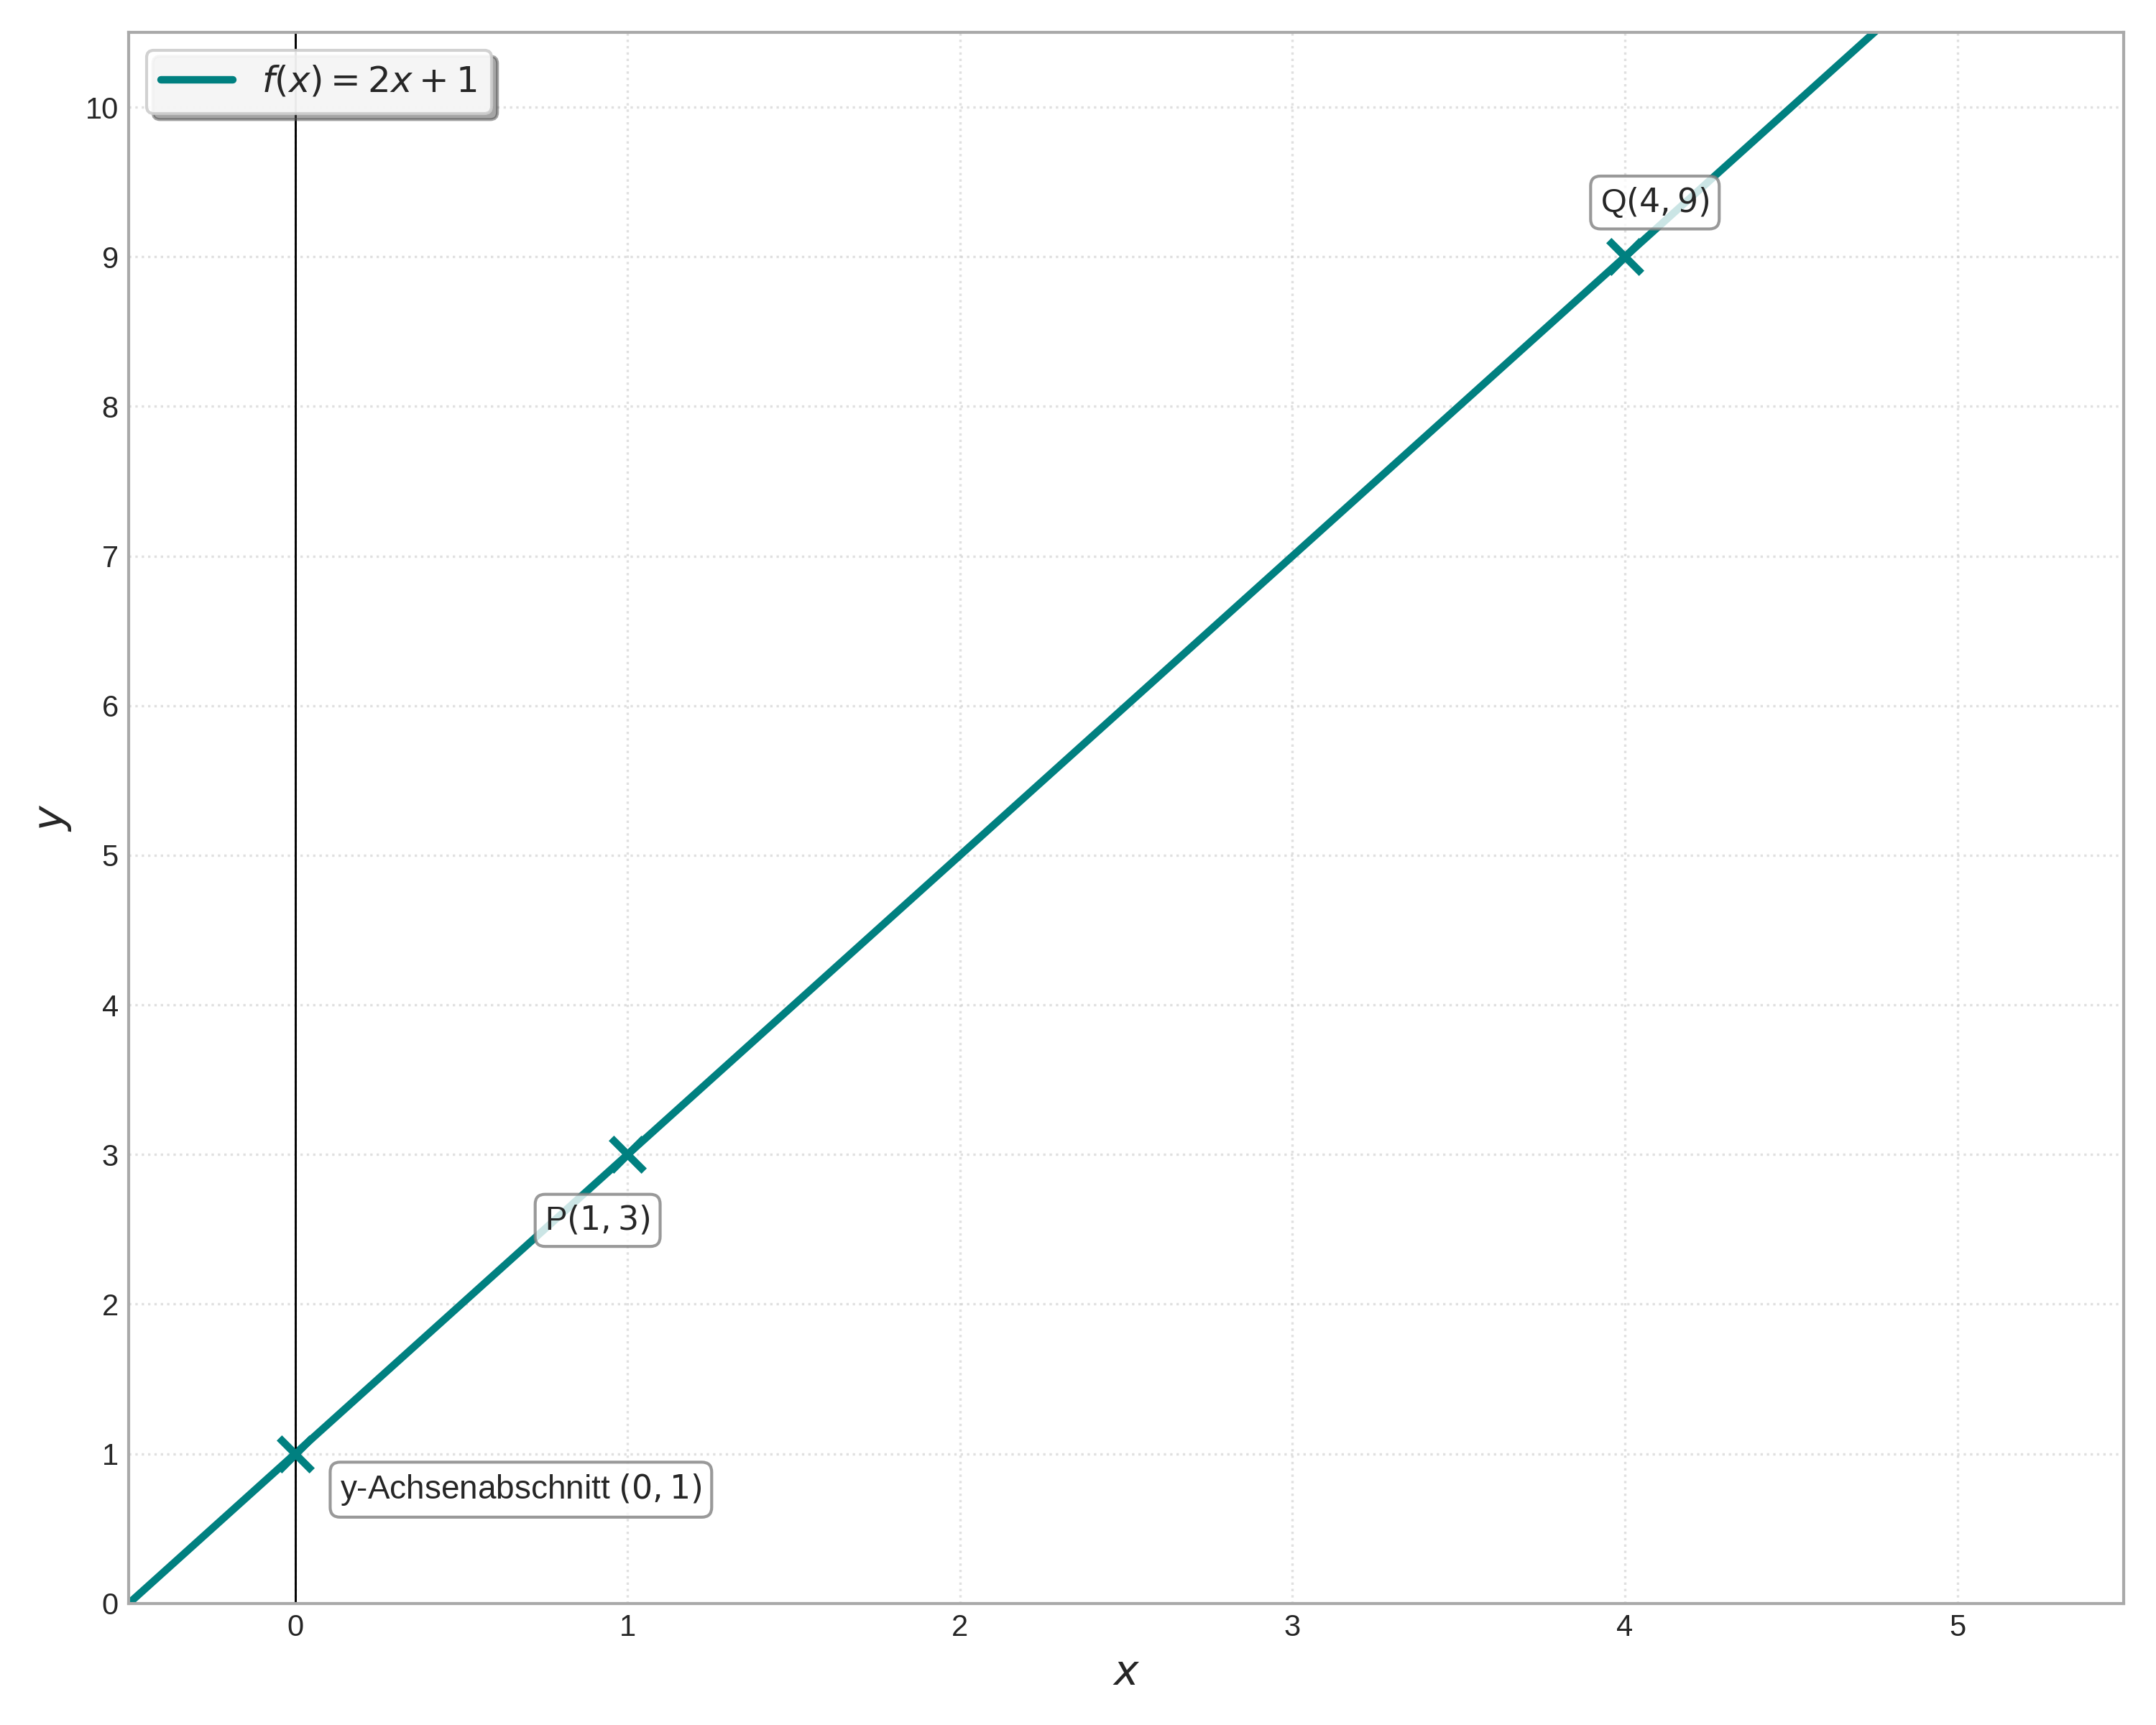
\includegraphics[width=0.8\textwidth]{grafiken/Lineare_Funktion_aus_2_Punkten.png}
    \captionof{figure}{Die Gerade $f(x)=2x+1$ durch die Punkte P und Q}
    \label{fig:gerade_aus_2_punkten}
\end{center}
% Der Text geht hier direkt weiter

\end{beispielumgebung}

Jetzt eine Aufgabe für dich, um das Verfahren zu üben.

\begin{aufgabenumgebung}{Lineare Funktionen umfassend bestimmen und analysieren}

\textbf{Teil 1: Gerade mit positiver Steigung} \\
Gegeben sind die Punkte $C(-2|0)$ und $D(2|8)$, durch die eine lineare Funktion $f(x) = ax+b$ verläuft.

\begin{enumerate}[label=(\alph*)]
    \item \textbf{Steigung berechnen:} Berechne die Steigung $a$ der Geraden durch die Punkte C und D.
    \item \textbf{Y-Achsenabschnitt berechnen:} Bestimme den y-Achsenabschnitt $b$ der Geraden.
    \item \textbf{Funktionsgleichung aufstellen:} Gib die vollständige Funktionsgleichung $f(x)$ an.
    \item \textbf{Nullstelle bestimmen:} Berechne die Nullstelle $x_N$ der Funktion $f(x)$. Welcher der gegebenen Punkte entspricht der Nullstelle?
    \item \textbf{Funktionswerte berechnen:}
        \begin{itemize}
            \item Welchen Wert hat $f(0)$? Was sagt dieser Wert über den Graphen aus?
            \item Berechne $f(1)$.
        \end{itemize}
    \item \textbf{Argument für einen Funktionswert finden:} Für welchen Wert von $x$ gilt $f(x) = 6$?
    \item \textbf{Punktprobe:} Liegt der Punkt $P(3|10)$ auf der Geraden? Begründe deine Antwort rechnerisch.
    \item \textbf{Skizze und Überprüfung:} Zeichne den Graphen der Funktion $f(x)$ in ein Koordinatensystem. Markiere die Punkte C und D sowie den y-Achsenabschnitt und die Nullstelle. Überprüfe anhand deiner Zeichnung, ob deine berechneten Werte für $a$ (Steigungsdreieck) und $b$ plausibel sind.
    \item \textbf{Vorzeichen der Funktionswerte:} Was kannst du über das Vorzeichen der Funktionswerte $f(x)$ sagen für $x$-Werte, die kleiner als die Nullstelle sind ($x < x_N$), und für $x$-Werte, die größer als die Nullstelle sind ($x > x_N$)? Begründe dies anhand der Steigung und der Nullstelle.
\end{enumerate}

\bigskip % Fügt einen größeren vertikalen Abstand ein

\textbf{Teil 2: Gerade mit negativer Steigung} \\
Gegeben sind die Punkte $E(-1|3)$ und $F(1|-1)$, durch die eine lineare Funktion $g(x) = ax+b$ verläuft.

\begin{enumerate}[label=(\alph*)]
    \item \textbf{Steigung berechnen:} Berechne die Steigung $a$ der Geraden durch die Punkte E und F.
    \item \textbf{Y-Achsenabschnitt berechnen:} Bestimme den y-Achsenabschnitt $b$ der Geraden.
    \item \textbf{Funktionsgleichung aufstellen:} Gib die vollständige Funktionsgleichung $g(x)$ an.
    \item \textbf{Nullstelle bestimmen:} Berechne die Nullstelle $x_N$ der Funktion $g(x)$.
    \item \textbf{Funktionswerte berechnen:}
        \begin{itemize}
            \item Welchen Wert hat $g(0)$? Was sagt dieser Wert über den Graphen aus?
            \item Berechne $g(3)$.
        \end{itemize}
    \item \textbf{Argument für einen Funktionswert finden:} Für welchen Wert von $x$ gilt $g(x) = 7$?
    \item \textbf{Punktprobe:} Liegt der Punkt $Q(0.5|0)$ auf der Geraden? Begründe deine Antwort rechnerisch. (Tipp: Vergleiche mit deiner Berechnung aus Teil d)).
    \item \textbf{Skizze und Überprüfung:} Zeichne den Graphen der Funktion $g(x)$ in ein Koordinatensystem. Markiere die Punkte E und F sowie den y-Achsenabschnitt und die Nullstelle. Überprüfe anhand deiner Zeichnung, ob deine berechneten Werte für $a$ (Ist die Gerade fallend? Wie ist das Steigungsdreieck?) und $b$ plausibel sind.
    \item \textbf{Vorzeichen der Funktionswerte:} Was kannst du über das Vorzeichen der Funktionswerte $g(x)$ sagen für $x$-Werte, die kleiner als die Nullstelle sind ($x < x_N$), und für $x$-Werte, die größer als die Nullstelle sind ($x > x_N$)? Begründe dies anhand der (negativen) Steigung und der Nullstelle.
\end{enumerate}
\end{aufgabenumgebung}

\subsubsection{Nullstellen linearer Funktionen – Wo die Gerade die x-Achse trifft}
Ein wichtiger Punkt einer Funktion ist ihre \textbf{Nullstelle}. Das ist der x-Wert, an dem der Funktionswert $f(x)$ gleich Null ist. Grafisch ist das der \textbf{Schnittpunkt der Geraden mit der x-Achse}.

\begin{merksatzumgebung}{Nullstelle einer linearen Funktion berechnen}
Um die Nullstelle $x_N$ einer linearen Funktion $f(x) = ax+b$ zu finden, setzt du den Funktionsterm gleich Null und löst nach $x$ auf:
\[ f(x_N) = 0 \]
\[ ax_N + b = 0 \]
Wenn $a \neq 0$ ist, kannst du die Gleichung umformen:
\begin{center}
\begin{tabular}{r @{\,} c @{\,} l @{\quad\quad} l}
$ax_N + b$ & $=$ & $0$ & $| -b$ \\
$ax_N$ & $=$ & $-b$ & $| :a \quad (\text{falls } a \neq 0)$ \\
$x_N$ & $=$ & $-\frac{b}{a}$ & \\
\end{tabular}
\end{center}
Die Nullstelle ist also $x_N = -b/a$. Der Punkt auf der x-Achse ist $N(-b/a | 0)$.

\textbf{Sonderfälle:}
\begin{itemize}
    \item \textbf{Fall 1: $a \neq 0$ und $b=0$ (proportionale Funktion $f(x)=ax$)}
    Dann ist $x_N = -0/a = 0$. Die Nullstelle ist im Ursprung $(0|0)$. Die Gerade geht durch den Ursprung.
    \item \textbf{Fall 2: $a = 0$ (konstante Funktion $f(x)=b$)}
    \begin{itemize}
        \item Wenn $b \neq 0$ (z.B. $f(x)=3$): Die Gleichung $b=0$ ist ein Widerspruch. Die Gerade ist parallel zur x-Achse und schneidet sie nie. Es gibt \textbf{keine Nullstelle}.
        \item Wenn $b = 0$ (also $f(x)=0$): Die Gleichung $0=0$ ist immer wahr. Die Gerade ist die x-Achse selbst. Es gibt \textbf{unendlich viele Nullstellen} (jeder x-Wert ist eine Nullstelle).
    \end{itemize}
\end{itemize}
\end{merksatzumgebung}

\begin{beispielumgebung}{Nullstelle berechnen}
Gegeben ist die Funktion $f(x) = 2x - 4$.
Wir suchen die Nullstelle, also setzen wir $f(x)=0$:
\begin{center}
\begin{tabular}{r @{\,} c @{\,} l @{\quad\quad} l}
$2x - 4$ & $=$ & $0$ & $| +4$ \\
$2x$ & $=$ & $4$ & $| :2$ \\
$x$ & $=$ & $2$ & \\
\end{tabular}
\end{center}
Die Nullstelle ist $x_N=2$. Der Schnittpunkt mit der x-Achse ist $N(2|0)$.
Mit der Formel: $x_N = -b/a = -(-4)/2 = 4/2 = 2$. Passt!
\end{beispielumgebung}

\begin{aufgabenumgebung}{Nullstellen finden}
Berechne die Nullstellen der folgenden linearen Funktionen. Gib auch den Schnittpunkt mit der x-Achse an.
\begin{enumerate}
    \item $f(x) = 3x + 6$
    \item $g(x) = -0.5x + 2$
    \item $h(x) = 4x$
    \item $k(x) = 5$ (Was passiert hier?)
\end{enumerate}
\end{aufgabenumgebung}

\subsubsection{Wertetabellen erstellen und nutzen}
Eine \textbf{Wertetabelle} ist eine Tabelle, die zu ausgewählten x-Werten die zugehörigen y-Werte (Funktionswerte) einer Funktion auflistet. Sie ist sehr nützlich, um:
\begin{itemize}
    \item Einen ersten Überblick über den Verlauf der Funktion zu bekommen.
    \item Punkte zu sammeln, um den Graphen der Funktion (hier eine Gerade) zu zeichnen.
    \item Spezifische Funktionswerte schnell nachzuschlagen.
\end{itemize}

\begin{merksatzumgebung}{Wertetabelle erstellen}
So erstellst du eine Wertetabelle für eine Funktion $f(x)$:
\begin{enumerate}
    \item \textbf{Wähle x-Werte aus:} Entscheide dich für einige x-Werte, für die du die Funktionswerte berechnen möchtest. Oft wählt man ganze Zahlen rund um den Ursprung (z.B. -2, -1, 0, 1, 2) oder Werte, die für eine Anwendungsaufgabe relevant sind.
    \item \textbf{Berechne die y-Werte:} Setze jeden gewählten x-Wert in die Funktionsgleichung $f(x)$ ein und berechne den zugehörigen y-Wert.
    \item \textbf{Trage die Wertepaare in eine Tabelle ein:}
\end{enumerate}
\end{merksatzumgebung}

\begin{beispielumgebung}{Wertetabelle für $f(x) = 0.5x + 1$}
Wir erstellen eine Wertetabelle für die Funktion $f(x) = 0.5x + 1$ für die x-Werte -2, -1, 0, 1, 2.

\begin{itemize}
    \item $x = -2 \implies f(-2) = 0.5 \cdot (-2) + 1 = -1 + 1 = 0$
    \item $x = -1 \implies f(-1) = 0.5 \cdot (-1) + 1 = -0.5 + 1 = 0.5$
    \item $x =  0 \implies f(0)  = 0.5 \cdot 0 + 1 = 0 + 1 = 1$ (Das ist der y-Achsenabschnitt!)
    \item $x =  1 \implies f(1)  = 0.5 \cdot 1 + 1 = 0.5 + 1 = 1.5$
    \item $x =  2 \implies f(2)  = 0.5 \cdot 2 + 1 = 1 + 1 = 2$
\end{itemize}

Die Wertetabelle sieht dann so aus:
\begin{center}
\begin{tabular}{c|c}
$x$ & $f(x) = 0.5x + 1$ \\
\hline
-2  & 0 \\
-1  & 0.5 \\
0   & 1 \\
1   & 1.5 \\
2   & 2 \\
\end{tabular}
\captionof{table}{Wertetabelle für $f(x)=0.5x+1$}
\end{center}
Mit diesen Punkten $(-2|0)$, $(-1|0.5)$, $(0|1)$, $(1|1.5)$, $(2|2)$ könntest du nun die Gerade zeichnen. Für eine Gerade reichen eigentlich zwei Punkte, aber eine Wertetabelle mit mehr Punkten gibt mehr Sicherheit beim Zeichnen und hilft, Rechenfehler zu entdecken.
\end{beispielumgebung}

\begin{aufgabenumgebung}{Deine Wertetabelle}
Erstelle eine Wertetabelle für die Funktion $g(x) = -2x + 3$ für die x-Werte von -3 bis 3 in Einerschritten. Zeichne anschließend den Graphen der Funktion mithilfe der Punkte aus deiner Wertetabelle.
\end{aufgabenumgebung}

\subsubsection{Einen x-Wert oder y-Wert bestimmen}
Manchmal ist ein x-Wert gegeben und der zugehörige y-Wert (Funktionswert) ist gesucht. Manchmal ist es umgekehrt: ein y-Wert ist bekannt und man möchte wissen, welcher x-Wert dazu gehört.

\begin{merksatzumgebung}{x- oder y-Wert bestimmen}
Gegeben sei eine lineare Funktion $f(x) = ax+b$.
\begin{itemize}
    \item \textbf{y-Wert (Funktionswert) zu einem gegebenen x-Wert bestimmen:}
    Setze den gegebenen x-Wert einfach in die Funktionsgleichung ein und berechne $f(x)$.
    Beispiel: $f(x)=2x+1$. Was ist $f(3)$? $f(3) = 2 \cdot 3 + 1 = 6+1=7$. Der y-Wert ist 7. Der Punkt ist $(3|7)$.

    \item \textbf{x-Wert zu einem gegebenen y-Wert (Funktionswert) bestimmen:}
    Setze den gegebenen y-Wert für $f(x)$ in die Funktionsgleichung ein: $y_{gegeben} = ax+b$.
    Löse diese Gleichung dann nach $x$ auf:
    \begin{center}
    \begin{tabular}{r @{\,} c @{\,} l @{\quad\quad} l}
    $y_{gegeben}$ & $=$ & $ax+b$ & $|-b$ \\
    $y_{gegeben} - b$ & $=$ & $ax$ & $|:a \quad (\text{falls } a \neq 0)$ \\
    $\frac{y_{gegeben} - b}{a}$ & $=$ & $x$ & \\
    \end{tabular}
    \end{center}
    Beispiel: $f(x)=2x+1$. Für welchen x-Wert ist $f(x)=9$?
    \begin{center}
    \begin{tabular}{r @{\,} c @{\,} l @{\quad\quad} l}
    $9$ & $=$ & $2x+1$ & $|-1$ \\
    $8$ & $=$ & $2x$ & $|:2$ \\
    $4$ & $=$ & $x$ & \\
    \end{tabular}
    \end{center}
    Der gesuchte x-Wert ist 4. Der Punkt ist $(4|9)$.
\end{itemize}
\end{merksatzumgebung}

Diese beiden Operationen sind grundlegend im Umgang mit Funktionen.

\begin{aufgabenumgebung}{Umgang mit linearen Funktionen: Werte und Schnittpunkte}

\textbf{Teil 1: Funktion $f(x) = -3x + 7$} \\
Gegeben ist die Funktion $f(x) = -3x + 7$.
\begin{enumerate}[label=(\alph*)]
    \item Berechne $f(-2)$, $f(0)$ und $f(4)$.
    \item Für welchen Wert von $x$ gilt $f(x) = 10$?
    \item Für welchen Wert von $x$ gilt $f(x) = -5$?
    \item An welcher Stelle schneidet der Graph die y-Achse? An welcher die x-Achse (Nullstelle)?
\end{enumerate}

\bigskip % Fügt einen größeren vertikalen Abstand ein

\textbf{Teil 2: Funktion $g(x) = \frac{1}{2}x - 1$} \\
Gegeben ist die Funktion $g(x) = \frac{1}{2}x - 1$.
\begin{enumerate}[label=(\alph*)]
    \item Berechne $g(-4)$, $g(0)$ und $g(6)$.
    \item Für welchen Wert von $x$ gilt $g(x) = 3$?
    \item Für welchen Wert von $x$ gilt $g(x) = -2.5$?
    \item An welcher Stelle schneidet der Graph die y-Achse? An welcher die x-Achse (Nullstelle)?
\end{enumerate}

\bigskip % Fügt einen größeren vertikalen Abstand ein

\textbf{Teil 3: Funktion $h(x) = -4x$} \\
Gegeben ist die Funktion $h(x) = -4x$.
\begin{enumerate}[label=(\alph*)]
    \item Berechne $h(-1.5)$, $h(0)$ und $h(2.5)$.
    \item Für welchen Wert von $x$ gilt $h(x) = 12$?
    \item Für welchen Wert von $x$ gilt $h(x) = -1$?
    \item An welcher Stelle schneidet der Graph die y-Achse? An welcher die x-Achse (Nullstelle)? Was ist hier besonders?
\end{enumerate}
\end{aufgabenumgebung}

% Dieser Block sollte in Kapitel 2: Lineare Funktionen eingefügt werden,
% z.B. nach dem Unterabschnitt 'Funktionsgleichung aufstellen' und 
% vor 'Anwendungsaufgaben – Lineare Funktionen im echten Leben'.

\subsubsection{Schnittpunkte zweier Geraden – Wo treffen sie sich?}
\label{subsubsec:schnittpunkte_geraden}

Oft haben wir nicht nur eine Gerade, sondern zwei (oder mehr) und möchten wissen, ob und wo sie sich schneiden. Der Schnittpunkt zweier Geraden $f(x)$ und $g(x)$ ist der Punkt $(x_S|y_S)$, der auf beiden Geraden liegt. Das bedeutet, an der Stelle $x_S$ müssen beide Funktionen denselben Funktionswert $y_S$ haben.

\begin{merksatzumgebung}{Schnittpunkt zweier Funktionen $f(x)$ und $g(x)$ berechnen}
Um den Schnittpunkt (oder die Schnittpunkte) zweier Funktionen $f(x)$ und $g(x)$ zu finden, gehst du wie folgt vor:
\begin{enumerate}
    \item \textbf{Funktionsterme gleichsetzen:}
    Setze die beiden Funktionsterme gleich:
    \[ f(x) = g(x) \]
    \item \textbf{Gleichung nach $x$ auflösen:}
    Löse die entstandene Gleichung nach der Variablen $x$. Der Wert (oder die Werte), den du für $x$ erhältst, ist die x-Koordinate des Schnittpunkts (der Schnittpunkte), $x_S$.
    \item \textbf{y-Koordinate berechnen:}
    Setze den gefundenen x-Wert $x_S$ in \textbf{eine der beiden ursprünglichen Funktionsgleichungen} ($f(x)$ oder $g(x)$ – es ist egal welche, da der Punkt ja auf beiden liegen soll) ein, um die zugehörige y-Koordinate $y_S$ zu berechnen.
    \[ y_S = f(x_S) \quad \text{oder} \quad y_S = g(x_S) \]
    \item \textbf{Schnittpunkt angeben:}
    Der Schnittpunkt ist $S(x_S|y_S)$.
\end{enumerate}
Zwei nicht-parallele Geraden haben immer genau einen Schnittpunkt. Parallele Geraden haben keinen Schnittpunkt (wenn sie verschieden sind) oder unendlich viele (wenn sie identisch sind).
\end{merksatzumgebung}

\begin{beispielumgebung}{Schnittpunkt zweier Geraden berechnen}
Gegeben sind die beiden linearen Funktionen:
$f(x) = 2x - 1$
$g(x) = -0.5x + 4$

Wir suchen den Schnittpunkt $S(x_S|y_S)$.

\textbf{Schritt 1: Funktionsterme gleichsetzen.}
$f(x) = g(x)$
$2x - 1 = -0.5x + 4$

\textbf{Schritt 2: Gleichung nach $x$ auflösen.}
Wir verwenden unsere Äquivalenzumformungen:
\begin{center}
\begin{tabular}{r @{\,} c @{\,} l @{\quad\quad} l}
$2x - 1$ & $=$ & $-0.5x + 4$ & $| +0.5x$ \\
$2.5x - 1$ & $=$ & $4$ & $| +1$ \\
$2.5x$ & $=$ & $5$ & $| :2.5$ \\
$x$ & $=$ & $2$ & \\
\end{tabular}
\end{center}
Die x-Koordinate des Schnittpunkts ist $x_S = 2$.

\textbf{Schritt 3: y-Koordinate berechnen.}
Wir setzen $x_S=2$ in eine der beiden ursprünglichen Gleichungen ein, z.B. in $f(x)$:
$y_S = f(2) = 2 \cdot 2 - 1 = 4 - 1 = 3$.
Zur Probe können wir auch in $g(x)$ einsetzen:
$y_S = g(2) = -0.5 \cdot 2 + 4 = -1 + 4 = 3$.
Das Ergebnis ist dasselbe, also $y_S=3$.

\textbf{Schritt 4: Schnittpunkt angeben.}
Der Schnittpunkt der beiden Geraden ist $S(2|3)$.

\begin{center}
    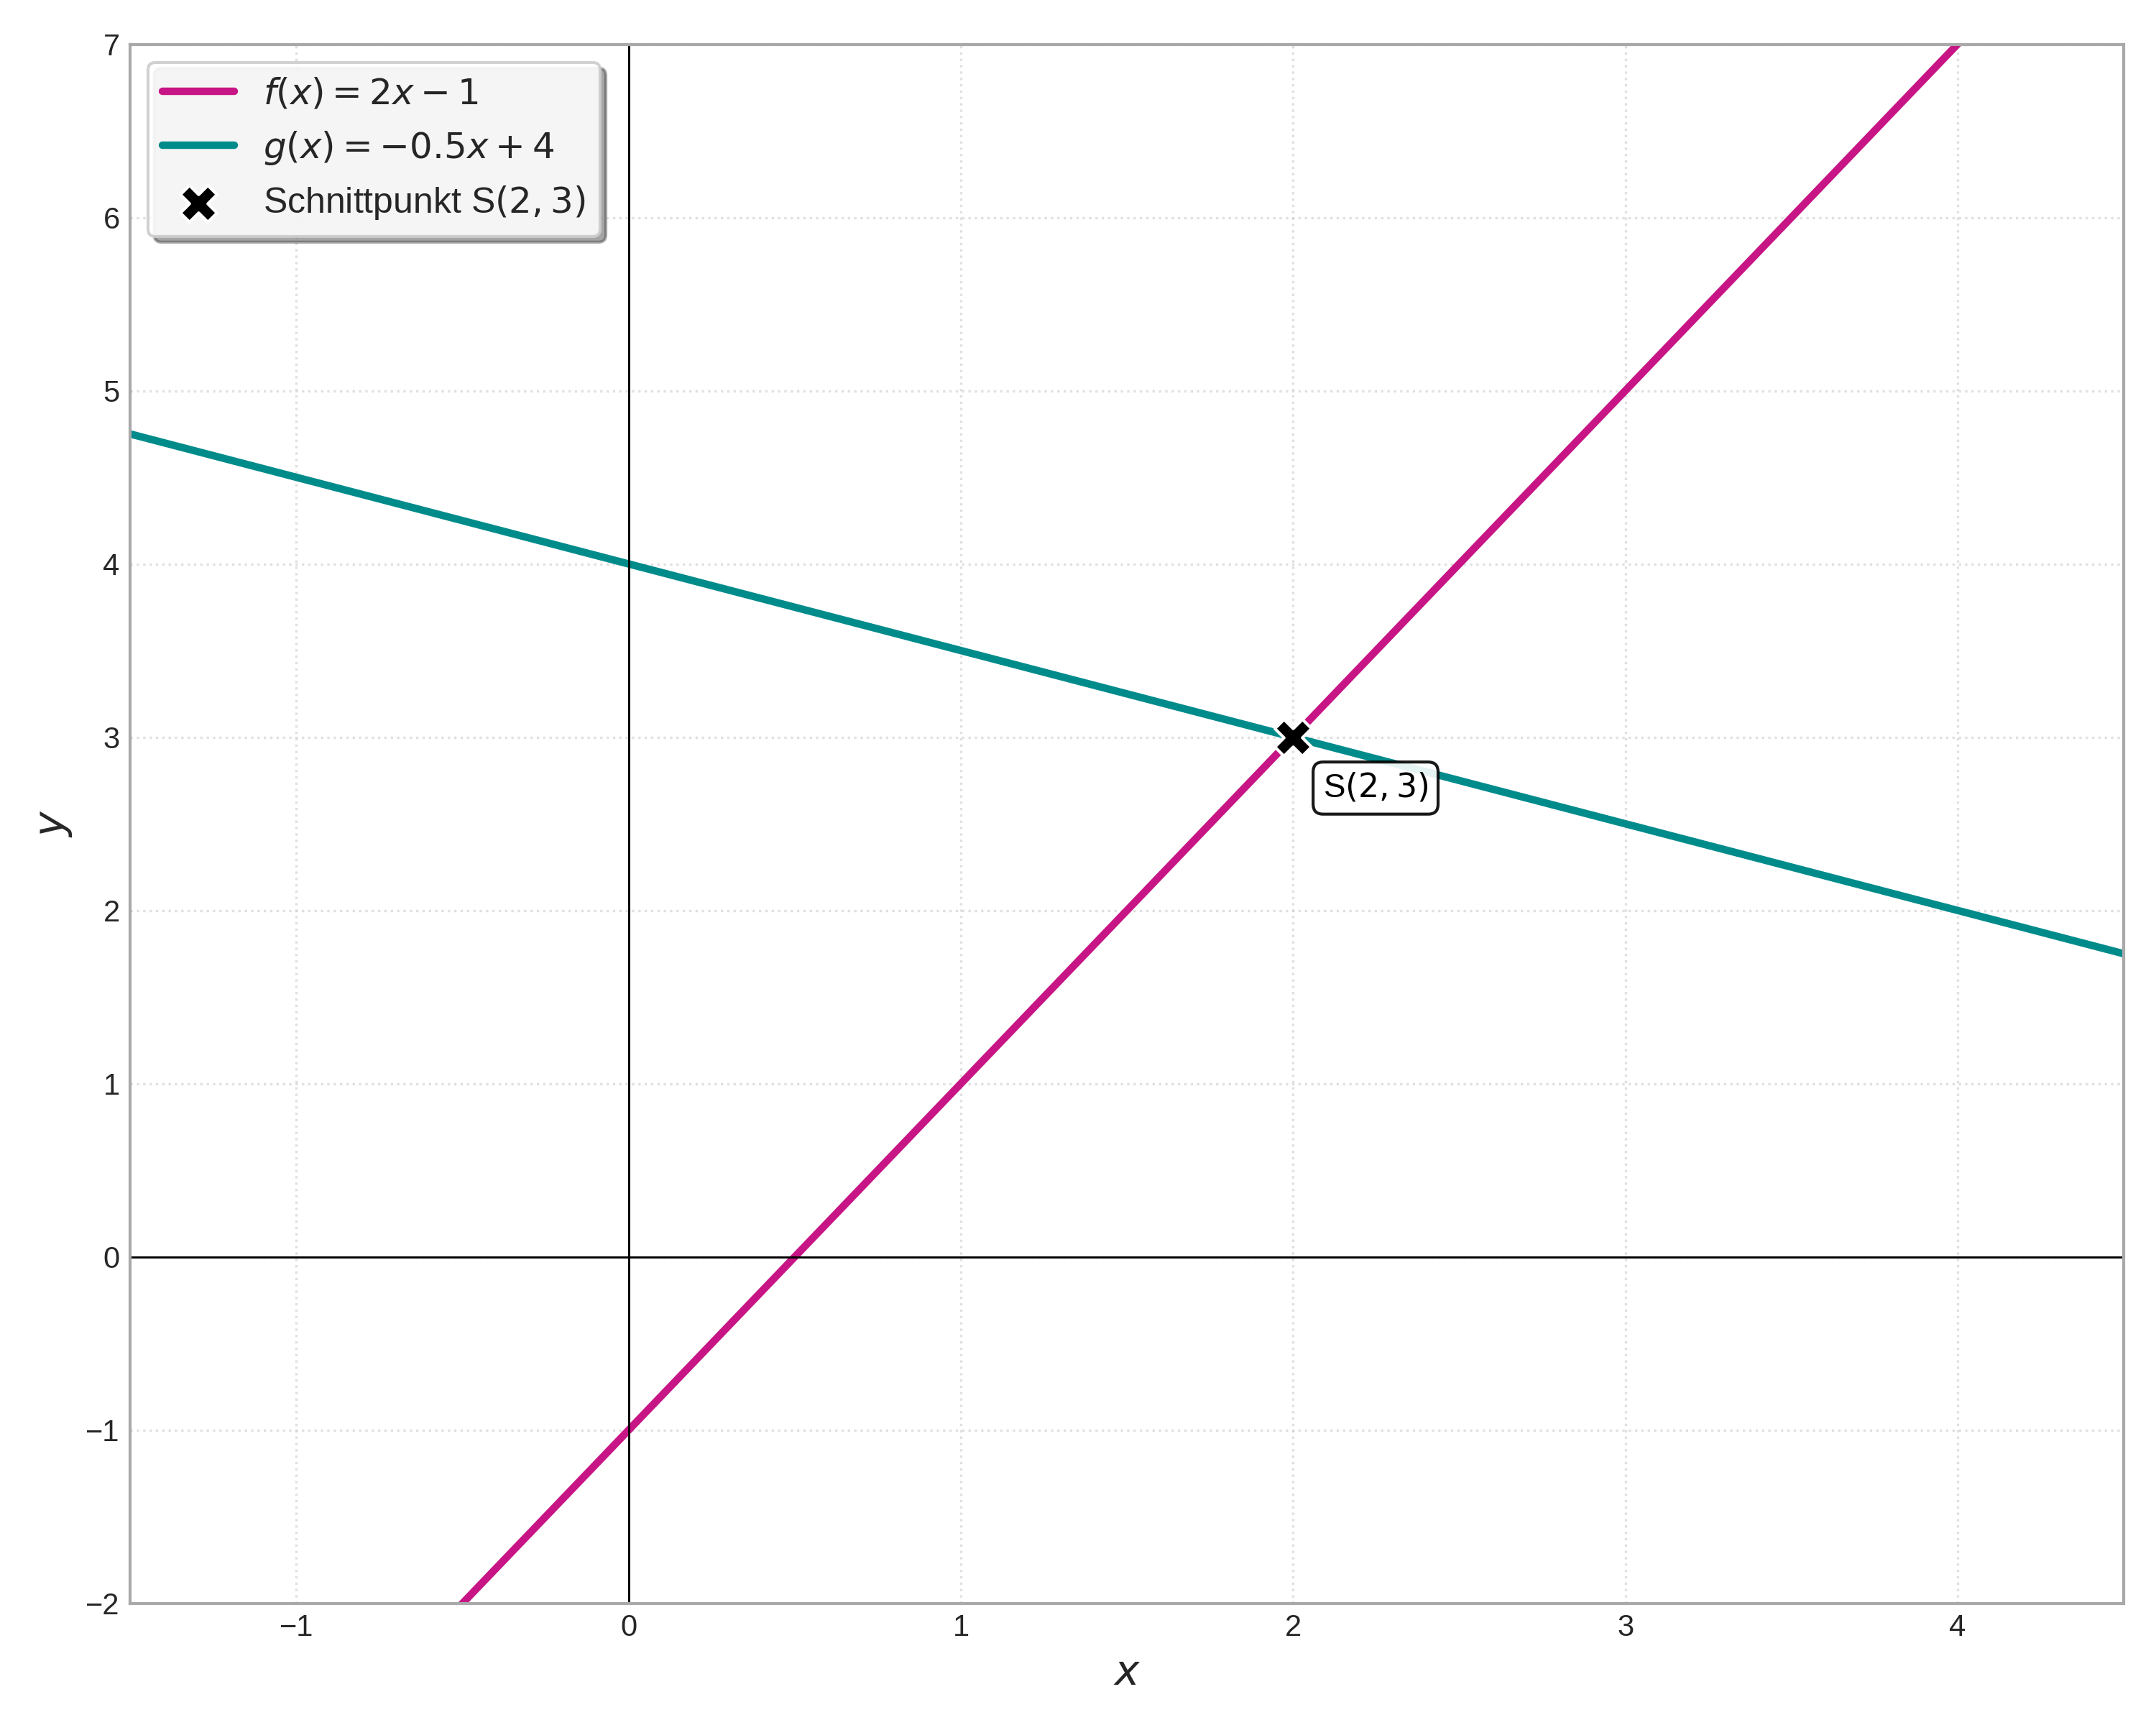
\includegraphics[scale = 0.5]{grafiken/Schnittpunkt_Zweier_Geraden.png}
    \captionof{figure}{Schnittpunkt der Geraden $f(x)=2x-1$ und $g(x)=-0.5x+4$}
    \label{fig:schnittpunkt_geraden_bsp}
\end{center}
% Der Text geht hier direkt weiter

\end{beispielumgebung}

\begin{aufgabenumgebung}{Schnittpunkte berechnen und zeichnen}
\begin{enumerate}
    \item Berechne den Schnittpunkt der folgenden Geradenpaare:
        \begin{itemize}
            \item $f(x) = x + 3$ und $g(x) = -2x + 9$
            \item $h(x) = 0.25x - 2$ und $k(x) = 0.25x + 1$ (Was stellst du hier fest? Wie liegen die Geraden zueinander?)
            \item $m(x) = \frac{1}{3}x + 1$ und $n(x) = -\frac{2}{3}x + 4$
        \end{itemize}
    \item Gegeben sind die Funktionen $f(x) = -x+5$ und $g(x) = 2x-1$.
        \begin{itemize}
            \item Berechne ihren Schnittpunkt $S$.
            \item Zeichne beide Geraden und ihren Schnittpunkt in ein Koordinatensystem.
        \end{itemize}
\end{enumerate}
\end{aufgabenumgebung}

\begin{warumwichtigumgebung}{Schnittpunkte}
Die Fähigkeit, Schnittpunkte von Funktionen zu berechnen, ist fundamental. Sie wird nicht nur bei Geraden benötigt, sondern auch bei Parabeln, Exponentialfunktionen und allen anderen Funktionstypen. Immer wenn gefragt wird, wann zwei Größen gleich sind oder wann sich zwei Prozesse treffen, führt dies mathematisch auf die Berechnung von Schnittpunkten. Die Nullstellenbestimmung ist ein Spezialfall davon: der Schnittpunkt mit der x-Achse (der Funktion $y=0$).
\end{warumwichtigumgebung}

% Hier würde dann der nächste Abschnitt des Kapitels 'Lineare Funktionen' folgen,
% z.B. 'Anwendungsaufgaben – Lineare Funktionen im echten Leben'.


Lineare Funktionen sind nicht nur abstrakte Gebilde, sondern haben viele praktische Anwendungen.

\subsection{Anwendungsaufgaben – Lineare Funktionen im echten Leben}

Viele reale Situationen lassen sich durch lineare Funktionen modellieren, zumindest näherungsweise. Oft gibt es eine Art 'Startwert' (entspricht $b$) und eine konstante Änderungsrate (entspricht $a$).

\begin{beispielumgebung}[Handyvertrag]{Kosten für einen Handyvertrag}
Ein Handyvertrag kostet monatlich eine Grundgebühr von 10 Euro. Jede SMS kostet zusätzlich 0,05 Euro.
Stelle eine Funktion auf, die die Gesamtkosten $K(x)$ in Abhängigkeit von der Anzahl $x$ der SMS beschreibt.

\textbf{Überlegung:}
\begin{itemize}
    \item Die Grundgebühr von 10 Euro zahlst du immer, auch wenn du keine SMS schreibst. Das ist dein fester Anteil, der nicht von $x$ abhängt. Das ist also der y-Achsenabschnitt $b=10$.
    \item Jede SMS kostet 0,05 Euro. Dieser Betrag wird mit der Anzahl $x$ der SMS multipliziert. Das ist also die Steigung $a=0,05$ (Kosten pro SMS).
\end{itemize}
\textbf{Funktionsgleichung:}
Die Kostenfunktion $K(x)$ lautet:
\[ K(x) = 0,05x + 10 \]
Hier ist $x$ die Anzahl der SMS und $K(x)$ die Gesamtkosten in Euro für einen Monat.

\textbf{Frage:} Wie viel kostet es, wenn man 100 SMS schreibt?
Wir setzen $x=100$ in die Funktion ein:
$K(100) = 0,05 \cdot 100 + 10 = 5 + 10 = 15$.
Antwort: Es kostet 15 Euro, wenn man 100 SMS schreibt.

\textbf{Frage:} Was bedeutet $K(0)$?
$K(0) = 0,05 \cdot 0 + 10 = 10$. Das sind die Kosten, wenn man keine SMS schreibt – also die reine Grundgebühr.
\end{beispielumgebung}

Solche Kostenfunktionen sind typische Anwendungsbeispiele.

\begin{aufgabenumgebung}{Taxifahrt}
Ein Taxifahrer verlangt eine Grundgebühr von 3,50 Euro für jede Fahrt. Zusätzlich kostet jeder gefahrene Kilometer 2 Euro.
\begin{enumerate}
    \item Stelle die Kostenfunktion $K(x)$ auf, wobei $x$ die Anzahl der gefahrenen Kilometer ist. Identifiziere $a$ und $b$ und erkläre ihre Bedeutung in diesem Kontext.
    \item Wie viel kostet eine Fahrt von 15 km?
    \item Du hast 25 Euro dabei. Wie viele Kilometer kannst du maximal fahren, wenn du den vollen Betrag ausgeben möchtest? (Tipp: Setze $K(x)=25$ und löse die Gleichung nach $x$ auf.)
    \item Zeichne den Graphen der Funktion $K(x)$ für $x$-Werte von 0 km bis 20 km. Wähle passende Einheiten für die Achsen.
\end{enumerate}
\end{aufgabenumgebung}

\begin{fehlerboxumgebung}{Typische Fehler bei linearen Funktionen}
\begin{itemize}
    \item \textbf{Vorzeichenfehler bei der Steigung:} Achte genau auf die Vorzeichen von $y_2, y_1, x_2, x_1$ bei der Formel $a = \frac{y_2-y_1}{x_2-x_1}$. Ein falsches Vorzeichen kehrt die Richtung der Geraden um!
    \item \textbf{Verwechslung von $a$ und $b$:} Die Steigung $a$ gibt an, wie steil es ist, der y-Achsenabschnitt $b$ ist der Startwert auf der y-Achse.
    \item \textbf{Fehler beim Umstellen von Gleichungen:} Übe das sichere Umstellen von Gleichungen (Äquivalenzumformungen), besonders wenn du $x$ bei gegebenem $y$ suchst oder $b$ aus einem Punkt und der Steigung.
    \item \textbf{Steigungsdreieck falsch ablesen/zeichnen:} Denke daran: $a = \frac{\Delta y}{\Delta x}$ (erst 'nach oben/unten', dann 'nach rechts').
\end{itemize}
\end{fehlerboxumgebung}

Hier sind noch ein paar weitere Übungen, um dein Verständnis zu festigen.

\begin{aufgabenumgebung}[labelA:LinUeb]{Lineare Funktionen – Übungen querbeet}
\begin{enumerate}
    \item \textbf{Paketversand:} Ein Paketversand kostet 5 Euro Grundgebühr. Jedes Kilogramm Gewicht kostet zusätzlich 1,50 Euro.
        \begin{itemize}
            \item Wie lautet die Kostenfunktion $K(g)$, wenn $g$ das Gewicht in Kilogramm ist?
            \item Was kostet ein Paket, das 3,2 kg wiegt?
            \item Ein Paket kostet 15,50 Euro. Wie schwer war es?
        \end{itemize}
    \item \textbf{Kerzenlänge:} Eine Kerze ist anfangs 20 cm lang. Pro Stunde brennt sie gleichmäßig 2,5 cm ab.
        \begin{itemize}
            \item Stelle eine Funktion $L(t)$ auf, die die Länge der Kerze nach $t$ Stunden beschreibt. (Achtung: Die Länge nimmt ab. Was bedeutet das für das Vorzeichen der Steigung $a$?)
            \item Wie lang ist die Kerze nach 3 Stunden?
            \item Nach wie vielen Stunden ist die Kerze komplett abgebrannt? (Das bedeutet, ihre Länge ist 0 cm.)
            \item Für welchen Zeitraum $t$ ist diese Funktion realistisch? (Definitionsbereich der Anwendung)
        \end{itemize}
    \item \textbf{Funktion aus Punkten:} Eine Gerade geht durch die Punkte $P_1(2|5)$ und $P_2(5|14)$. Bestimme ihre Funktionsgleichung $f(x)=ax+b$.
    \item \textbf{Funktion aus Steigung und Punkt:} Die Steigung einer Geraden ist $a = -2$. Die Gerade geht außerdem durch den Punkt $P(1|3)$. Bestimme den y-Achsenabschnitt $b$ und gib die vollständige Funktionsgleichung an. (Tipp: Setze $a$ und die Koordinaten von $P$ in $y=ax+b$ ein und löse nach $b$.)
\end{enumerate}
\end{aufgabenumgebung}

Das Konzept der Steigung als Änderungsrate ist fundamental und führt uns zu einem wichtigen Begriff in der Analysis.

\subsection{Die durchschnittliche Änderungsrate – Ein Vorgeschmack auf mehr}

Bei linearen Funktionen ist die Steigung $a$ konstant. Das bedeutet, die Änderungsrate ist immer gleich, egal welches Intervall man betrachtet. Bei kurvigen Funktionen ist das anders. Dort spricht man von der \textbf{durchschnittlichen Änderungsrate} über ein bestimmtes Intervall.

\begin{merksatzumgebung}[Durchschnittliche Änderungsrate]{Was ist das und wie berechnet man sie?}
Die durchschnittliche Änderungsrate einer Funktion $f$ im Intervall $[x_1, x_2]$ gibt an, wie stark sich der Funktionswert $f(x)$ \textbf{im Durchschnitt} ändert, wenn sich der $x$-Wert von $x_1$ nach $x_2$ ändert.
Sie ist nichts anderes als die \textbf{Steigung der Sekante} (eine Gerade, die durch die beiden Punkte $(x_1|f(x_1))$ und $(x_2|f(x_2))$ auf dem Funktionsgraphen geht).

Die Formel lautet:
\[ \text{Durchschnittliche Änderungsrate im Intervall } [x_1, x_2] = m_{Sekante} = \frac{f(x_2) - f(x_1)}{x_2 - x_1} = \frac{\Delta y}{\Delta x} \]
Du siehst, das ist genau die gleiche Formel wie für die Steigung $a$ einer linearen Funktion!
Bei \textbf{linearen Funktionen} ist die durchschnittliche Änderungsrate in jedem Intervall konstant und entspricht genau der Steigung $a$ der Geraden. Bei anderen (nicht-linearen) Funktionen ändert sich die durchschnittliche Änderungsrate jedoch, je nachdem, welches Intervall $[x_1, x_2]$ man wählt.
\end{merksatzumgebung}

Ein Beispiel aus dem Alltag macht das klarer.

\begin{beispielumgebung}[Kilometerstand eines Autos]{Durchschnittliche Fahrleistung}
Am 1. Mai (Tag 0 eines Beobachtungszeitraums) zeigt der Kilometerzähler eines Autos 10.000 km. Am 1. Oktober (nach 5 Monaten, also am Tag $5 \times 30 = 150$ ungefähr, oder einfacher: Monat 0 bis Monat 5) zeigt er 25.000 km.
Wie viele Kilometer ist das Auto \textbf{durchschnittlich} pro Monat gefahren?

Hier können wir die Monate als 'x-Werte' und die Kilometerstände als 'Funktionswerte' betrachten.
$x_1 = 0$ Monate (Startzeitpunkt)
$f(x_1) = 10.000$ km (Kilometerstand zu Beginn)

$x_2 = 5$ Monate (Endzeitpunkt)
$f(x_2) = 25.000$ km (Kilometerstand am Ende)

Die Veränderung der Monate ist $\Delta x = x_2 - x_1 = 5 - 0 = 5$ Monate.
Die Veränderung des Kilometerstandes ist $\Delta y = f(x_2) - f(x_1) = 25.000 \text{ km} - 10.000 \text{ km} = 15.000 \text{ km}$.

Die durchschnittliche Fahrleistung (Änderungsrate) ist:
\[ \frac{\Delta y}{\Delta x} = \frac{15.000 \text{ km}}{5 \text{ Monate}} = 3.000 \text{ km/Monat} \]
Das Auto ist also im Durchschnitt 3000 km pro Monat gefahren. Das heißt nicht, dass es jeden Monat genau 3000 km gefahren ist – mal mehr, mal weniger – aber im Schnitt über die 5 Monate waren es 3000 km/Monat.
\end{beispielumgebung}

Dieser Begriff ist sehr nützlich, um Veränderungen über Zeiträume zu analysieren.

\begin{aufgabenumgebung}{Deine durchschnittliche Rate}
Denke dir ein eigenes Beispiel aus dem Alltag aus, bei dem eine Größe sich über die Zeit oder eine andere Einheit verändert (z.B. Wasserverbrauch einer Familie über mehrere Tage, Wachstum einer Pflanze über Wochen, Temperaturänderung im Laufe eines Tages, Anzahl der gelesenen Seiten eines Buches über mehrere Abende).
\begin{enumerate}
    \item Beschreibe die Situation klar. Welche Größe ändert sich in Abhängigkeit von welcher anderen Größe?
    \item Lege zwei Messpunkte (Anfangswert mit zugehörigem 'x1' und Endwert mit zugehörigem 'x2') fest.
    \item Berechne die durchschnittliche Änderungsrate. Was sagt diese Rate in deinem Beispiel konkret aus? Welche Einheit hat sie?
\end{enumerate}
\end{aufgabenumgebung}

\begin{kurzknappumgebung}{Lineare Funktionen}
\begin{itemize}
    \item \textbf{Form:} $f(x) = ax+b$ (Graph ist eine Gerade).
    \item \textbf{$a$ = Steigung:} Gibt an, wie stark die Gerade steigt/fällt. $a = \frac{\Delta y}{\Delta x}$.
    \item \textbf{$b$ = y-Achsenabschnitt:} Schnittpunkt mit der y-Achse bei $(0|b)$.
    \item \textbf{Nullstelle $x_N$:} Schnittpunkt mit der x-Achse. Lösung von $ax+b=0 \implies x_N = -b/a$ (für $a \neq 0$).
    \item \textbf{Wertetabelle:} Hilft beim Zeichnen und Verstehen.
    \item \textbf{Durchschnittliche Änderungsrate:} Ist bei linearen Funktionen immer gleich der Steigung $a$.
\end{itemize}
\end{kurzknappumgebung}

\begin{infoboxumgebung}{Ausblick: Von der durchschnittlichen zur momentanen Änderungsrate}
Die durchschnittliche Änderungsrate betrachtet, wie der Name schon sagt, einen Durchschnitt über ein Intervall. In der \textbf{Differentialrechnung}, einem Kerngebiet der Analysis, wollen wir aber oft wissen, wie schnell sich etwas in einem \textbf{einzigen Moment} ändert. Das nennt man die \textbf{momentane Änderungsrate} oder auch die \textbf{Ableitung} einer Funktion an einer bestimmten Stelle.
Stell dir vor, du machst das Intervall $[x_1, x_2]$ immer kleiner und kleiner, sodass $x_2$ ganz nah an $x_1$ heranrückt. Was passiert dann mit der Steigung der Sekante? Sie nähert sich der Steigung der \textbf{Tangente} an den Graphen im Punkt $(x_1|f(x_1))$. Diese Tangentensteigung ist dann die momentane Änderungsrate. Das ist eine der faszinierendsten Ideen der Analysis, die wir später genauer untersuchen werden!
\begin{center}
    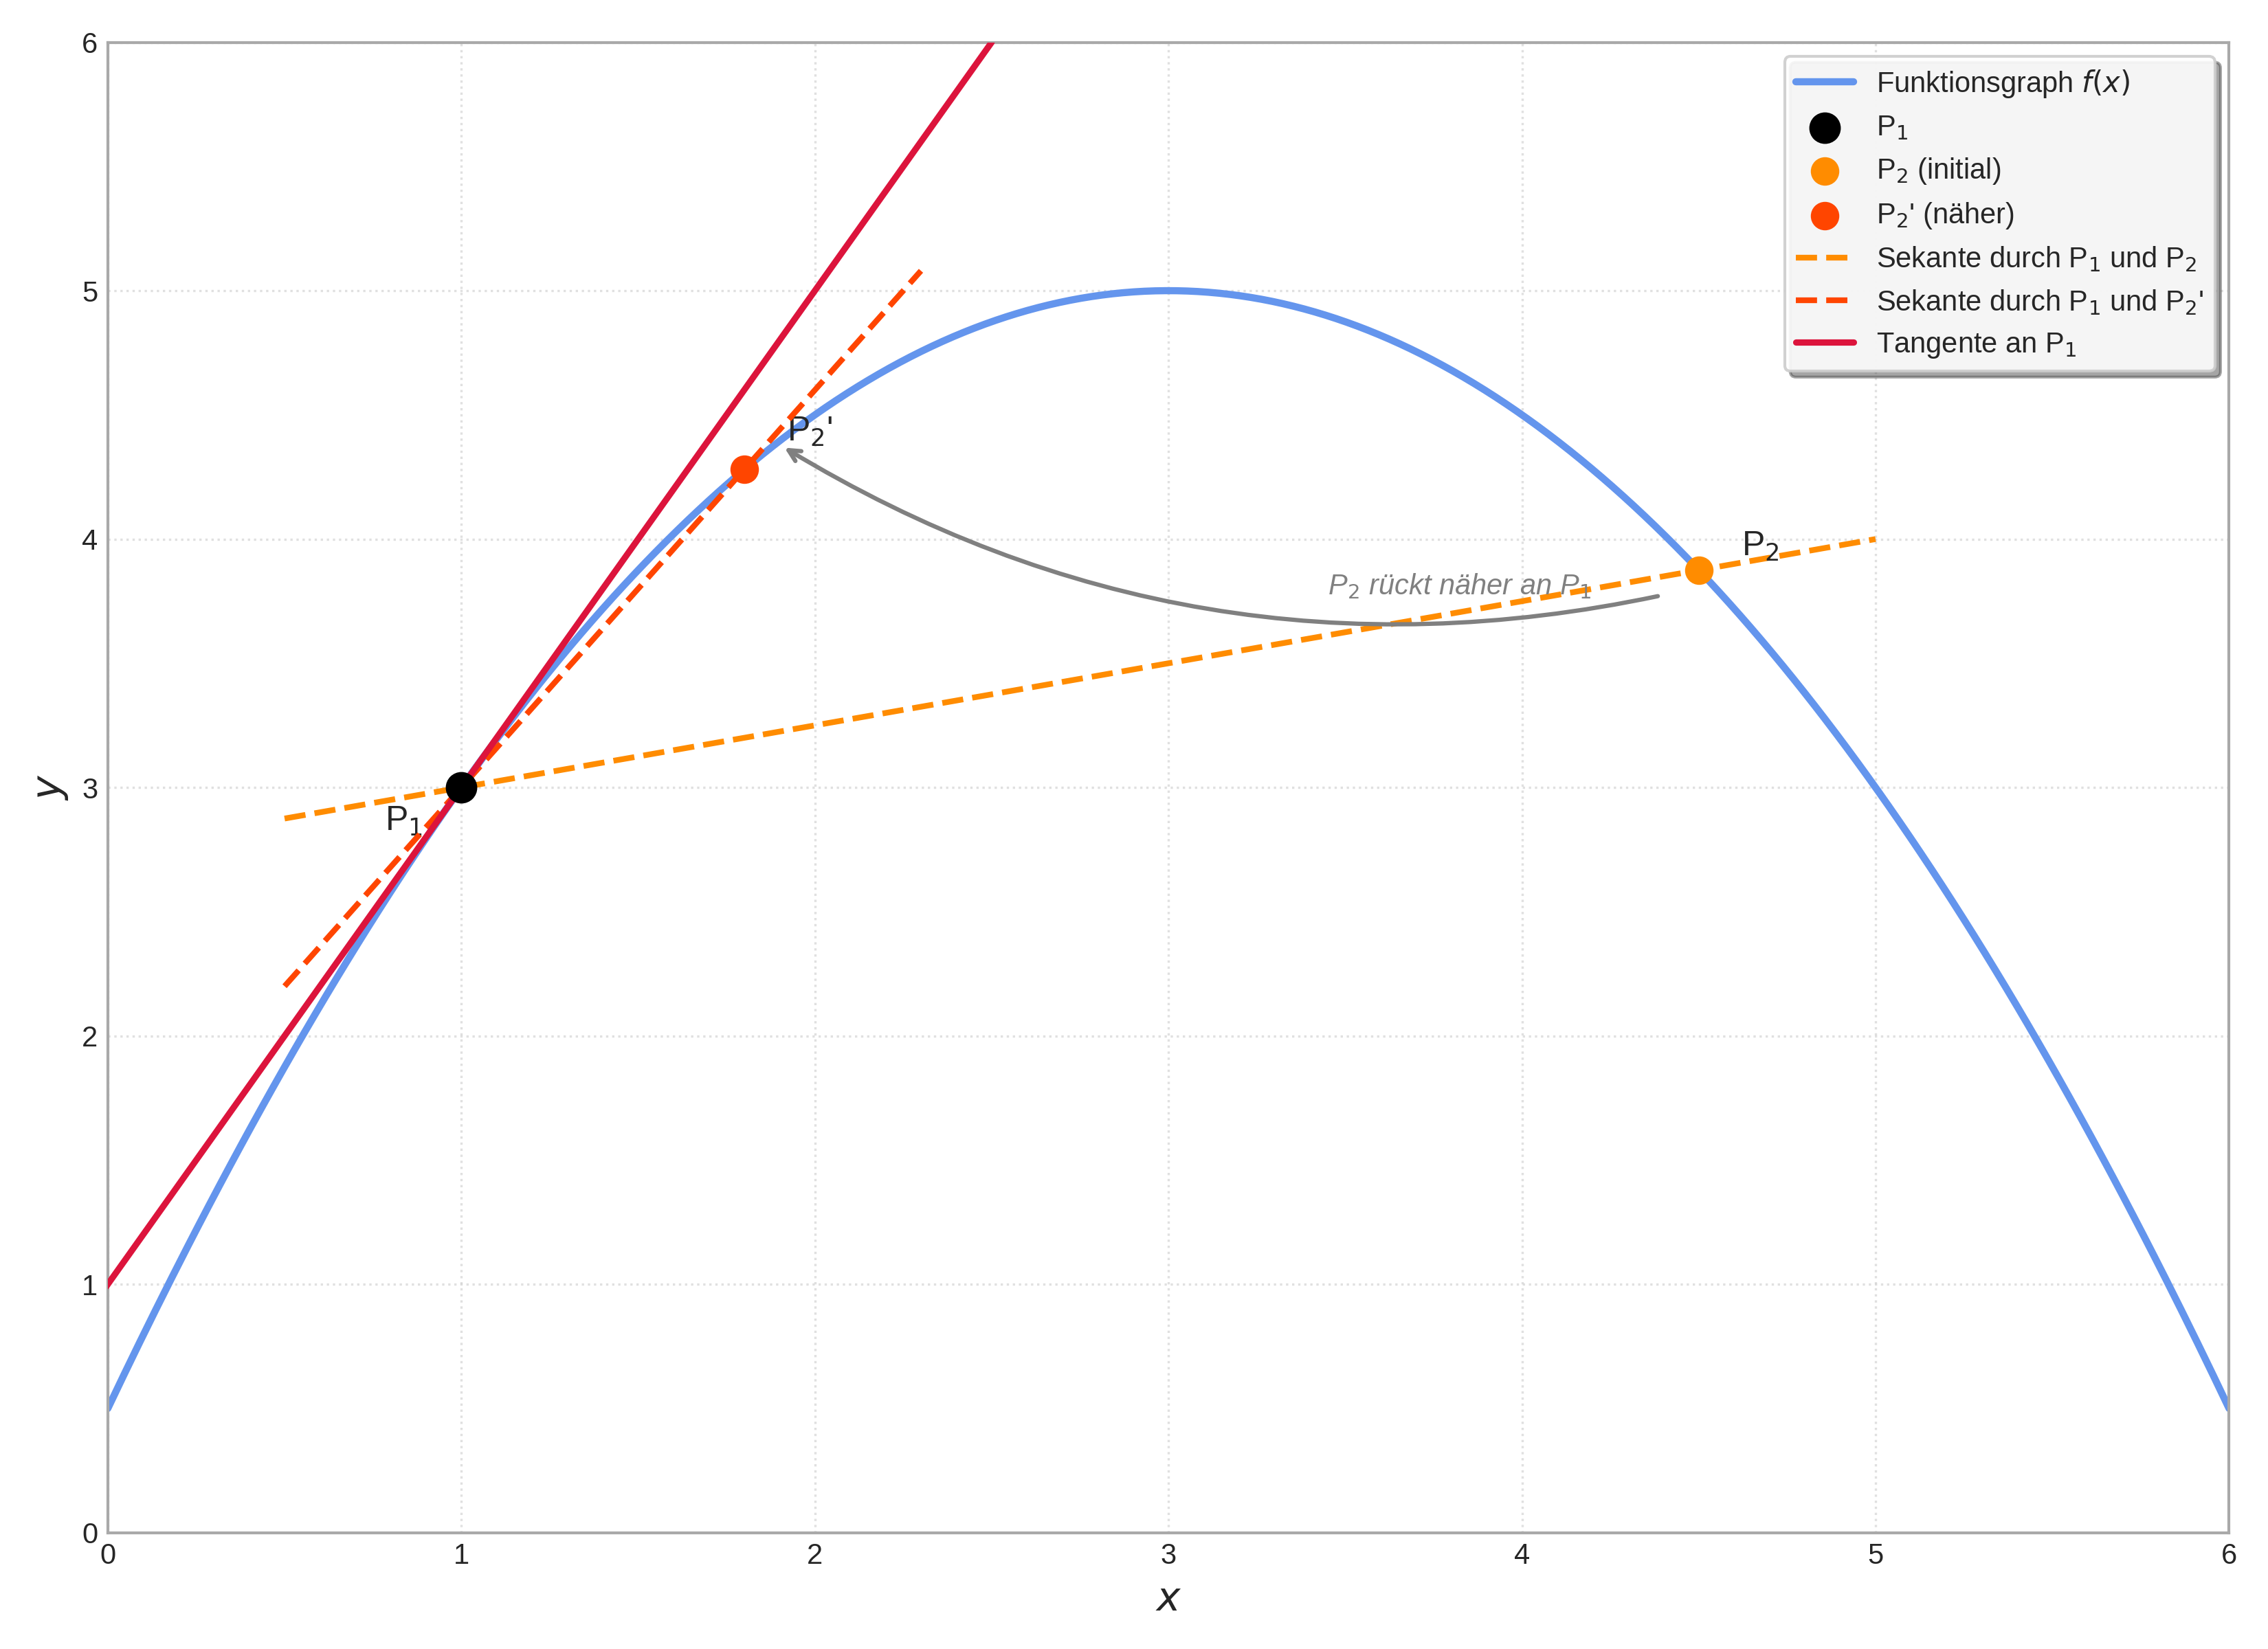
\includegraphics[width=0.8\textwidth]{grafiken/Sekante_zur_Tangente.png}
    \captionof{figure}{Von der Sekantensteigung zur Tangentensteigung}
    \label{fig:sekante_tangente}
\end{center}
% Der Text geht hier direkt weiter

\end{infoboxumgebung}


\begin{aufgabenumgebung}{Checkliste: Eigenschaften einer linearen Funktion analysieren}
Betrachte die lineare Funktion $f(x) = \frac{1}{2}x - 1$.
Bearbeite die folgenden Punkte, um dein Verständnis dieser Funktion zu überprüfen:

\begin{enumerate}[label=(\alph*)]
    \item \textbf{Nullstelle:} Berechne die Nullstelle $x_0$ der Funktion $f(x)$ (d.h. die Stelle, an der $f(x_0)=0$ ist).
    \item \textbf{Y-Achsenabschnitt:} Bestimme den Schnittpunkt mit der y-Achse (den y-Achsenabschnitt $b$). Welchen Wert hat die Funktion an der Stelle $x=0$?
    \item \textbf{Skizze:} Zeichne den Graphen der Funktion $f(x)$ sorgfältig in ein Koordinatensystem. Markiere deutlich die Nullstelle auf der x-Achse und den y-Achsenabschnitt auf der y-Achse.
    \item \textbf{Funktionswerte positiv/negativ:}
    \begin{itemize}
        \item Für welche $x$-Werte sind die Funktionswerte $f(x)$ \textbf{positiv} (d.h. der Graph verläuft oberhalb der x-Achse)? Gib den Bereich an.
        \item Für welche $x$-Werte sind die Funktionswerte $f(x)$ \textbf{negativ} (d.h. der Graph verläuft unterhalb der x-Achse)? Gib den Bereich an.
    \end{itemize}
    \item \textbf{Rolle der Steigung:} Wie hilft dir das Vorzeichen der Steigung $a = \frac{1}{2}$ dabei, die Bereiche aus Teil (d) schnell zu bestimmen, sobald du die Nullstelle kennst? Erkläre in eigenen Worten.
    \item \textbf{Rolle des y-Achsenabschnitts:} Betrachte den y-Achsenabschnitt $b=-1$. Hilft dir dieser Wert auch dabei, das Vorzeichen der Funktion in einem bestimmten Bereich (z.B. für $x$-Werte nahe Null) zu bestimmen? Begründe.
    \item \textbf{Wertebereich:} Der Wertebereich einer nicht-konstanten linearen Funktion ist die Menge aller reellen Zahlen $\mathbb{R}$. Wie kannst du das an deinem Graphen erkennen oder dir vorstellen, dass jeder y-Wert irgendwann einmal getroffen wird?
\end{enumerate}
\end{aufgabenumgebung}

\begin{aufgabenumgebung}{Checkliste: Verhalten linearer Funktionen verstehen und interpretieren}
Gegeben sei die lineare Funktion $g(x) = -2x + 4$.
Führe eine Analyse dieser Funktion anhand der folgenden Punkte durch:

\begin{enumerate}[label=(\alph*)]
    \item \textbf{Nullstelle und y-Achsenabschnitt:} Berechne die Nullstelle von $g(x)$ und gib den y-Achsenabschnitt an.
    \item \textbf{Skizze:} Zeichne den Graphen der Funktion $g(x)$. Achte darauf, die Achsenschnittpunkte klar zu kennzeichnen.
    \item \textbf{Vorzeichen der Funktionswerte:}
    \begin{itemize}
        \item In welchem Intervall ist $g(x) > 0$?
        \item In welchem Intervall ist $g(x) < 0$?
    \end{itemize}
    \item \textbf{Argumentation mit Steigung und Nullstelle:} Erkläre, wie du allein aus dem Vorzeichen der Steigung $a=-2$ und der Lage der Nullstelle $x_0$ schlussfolgern kannst, ob die Funktionswerte für $x$-Werte, die größer als die Nullstelle sind ($x > x_0$), positiv oder negativ sein müssen.
    \item \textbf{Vergleich mit dem y-Achsenabschnitt:} Bestätigt der y-Achsenabschnitt deine Überlegungen zum Vorzeichen der Funktion für $x=0$? Liegt $x=0$ in dem von dir bestimmten positiven oder negativen Bereich?
    \item \textbf{Gedankenexperiment:} Stell dir eine lineare Funktion $h(x)$ vor, von der du nur weißt: Ihre Steigung ist positiv ($a > 0$) und ihre Nullstelle ist ebenfalls positiv ($x_0 > 0$).
    \begin{itemize}
        \item Mache eine grobe Skizze, wie solch eine Funktion aussehen könnte.
        \item Welches Vorzeichen muss der y-Achsenabschnitt dieser Funktion $h(x)$ haben? Begründe deine Antwort mathematisch oder anhand deiner Skizze.
    \end{itemize}
\end{enumerate}
\end{aufgabenumgebung}